\newpage
\chapter{Analyse fonctionnelle des réplicons}\label{chap6true}
\lhead{\emph{Analyse fonctionnelle des réplicons}}\label{paranalysefunc}
	
	Pour caractériser les bases biologiques de la différentiation des types de réplicon, nous avons procédé à des analyses complémentaires en ne considérant plus comme variables les clusters d'homologues de protéines mais leurs annotations fonctionnelles. Chaque réplicon est ainsi décrit par une distribution de fonctions des STIG, qui sert de base à la comparaison/discrimination des réplicons. Un avantage de cette modalité de représentation est de réduire la dimensionalité des données. L'inconvénient, cependant, est que l'information liée aux homologies de séquence des protéines est perdue. Nous avons effectué trois types d'analyses fonctionnelles: i) la visualisation des réplicons et des génomes par les fonctions des clusters, ii) des analyses de régression de la distribution des fonctions selon le type de réplicon et de génome, et iii) des analyses de classification des réplicons et génomes.
	
\section{Jeux de données et notation}\label{pardonnee2}

\subsection{Notations}
Soient une protéine $p$ et son annotation $Ann(p)$ définie par la relation \ref{eqannot}, et un groupe de protéines $C$. On définit $Ann(C)$, l'annotation de $C$ par:
	 \begin{equation}
		Ann(C)=Ann(p) \iff N^{C}_{Ann(p)}=max\{N^{C}_{Ann(p_{i})}|\; p_{i} \in C\}
	\end{equation}
	où $N^{C}_{Ann(p)}$ est le nombre de fois que $Ann(p)$ apparaît dans $C$, tel que:
		 \begin{equation}
			N^{C}_{Ann(p)}=|\{Ann(p_{i})|\; p_{i} \in C \textrm{ et } Ann(p)=Ann(p_{i}) \}|
		\end{equation}

Soit un cluster de protéines $Cl$. On définit par $F$, son ensemble fonctionnel, tel que:
	\begin{equation}
		F^{Cl} = \{Ann(C)|\; C \in Cl \textrm{ et } Ann(C) \textrm{ unique} \}
	\end{equation}   

Soient $r$ un réplicon et $v_{r}$ son vecteur associé pour un clustering de protéines $Cl$ donné, défini par l'éq. \ref{eqvr}. On définit alors $v^{f}_{r}$, son vecteur fonctionnel tel que:
	\begin{equation}
		v^{f}_{r}=(N^{r}_{f_{1}},...,N^{r}_{f_{|F|}}),\; f \in F^{Cl}
	\end{equation}
où $N^{r}_{f}$ est défini par:
	\begin{equation}
		N^{r}_{f}=\sum_{\substack{{C \in Cl} \\{Ann(C)=f}}}N^{r}_{C}
	\end{equation}
avec $N^{r}_{C}$ défini par l'éq. \ref{eqvr}. \\

Pour un génome $g=\{r_{1},...,r_{|g|}\}$ (relation \ref{eqindiv}), on définit $v_{f}^{g}$ par:
	\begin{equation}
		v^{g}_{f}=(N^{g}_{f_{1}},...,N^{g}_{f_{|F|}}),\; f \in F
	\end{equation}
où $N^{g}_{f}$ est défini par:
	\begin{equation}
		N^{g}_{f}=\sum_{r \in g}N^{r}_{f}
	\end{equation}

Pour des ensembles de réplicons $R$ et de génomes $G$, on définit $V^{R}_{f}=\{v^{r}_{f}|r \in R\}$ et $V^{G}_{f}=\{v^{g}_{f}|g \in G\}$ similairement à l'éq. \ref{eqV}, ainsi que $\bar{V}^{R}_{f,n\_tax}$ similairement à l'éq. \ref{eqVnorm}. $\bar{V}^{G}_{f,n\_tax}$ est de plus défini par:
	\begin{equation}
		\bar{V}^{G}_{f,n\_tax}=\bar{V}^{Kl_{n\_tax}^{G^{\{monopartite\}}}}\cup\bar{V}^{Kl_{n\_tax}^{G^{\{multipartite\}}}}
	\end{equation}
où $G^{\{monopartite\}}$ est l'ensemble des génomes ne contenant pas de RECE et $G^{\{multipartite\}}$ est l'ensemble des génomes contenant au moins un réplicon annoté comme RECE. \\

Les annotations utilisées pour les protéines de $P_{ref}$ correspondent aux annotations de KEGG (Appendice \ref{AppendiceB}) et à nos annotations des groupes ACLAME (Appendice \ref{AppendiceC}).


\subsection{Dimension des données}
	Les 6096 clusters de protéines ($Cl$) obtenus par TRIBE-MCL avec une granularité $gr = 4$ ont été annotés par \textbf{117} fonctions (71 de KEGG et 46 de ACLAME). \textbf{2720} génomes bactériens ont de plus été formé à partir des données. Similairement aux analyses précédentes, l'indice taxonomique \textit{n\_tax} de normalisation des données choisi est le \textit{genre}. Les caractéristiques des données sont présentées Table \ref{tabdim2}.
	
\begin{table}[H]
	\caption[Dimension des données fonctionnelles]{Dimension des données.}\label{tabdim2}
	\begin{center}
	\begin{tabular}{c|c|c}
	\textbf{Ensemble de données} & \textbf{Matrice} & \textbf{Taille} \\
	\hline
	$Cl$ & - & 6096 \\
	$F^{Cl}$ & - & 117 \\
	$V^{R}_{f} $ & $M^{V^{R}_{f}}$ & (4928,117)  \\
	$\bar{V}^{R}_{f,genre} $ & $M^{\bar{V}^{R}_{f,genre}}$ & (851,117)  \\
	$V^{G}_{f} $ & $M^{V^{G}_{f}}$ & (2720,117)  \\
	$\bar{V}^{G}_{f,genre}$ & $M^{\bar{V}^{G}_{f,genre}}$ & (584,117)  \\
	\end{tabular}
	\end{center}
\end{table}	

	 
\section{Discrimination fonctionnelle des réplicons} \label{pardiscriminfuncrepl}  
	Une ségrégation fonctionnelle d'un certain groupe de réplicons est potentiellement le témoin de la spécificité fonctionnelle de ce groupe par rapport aux autres réplicons. L'objectif sous-jacent est alors d'identifier des groupes de RECE, \textbf{témoins de l'adaptation fonctionnelle de ces éléments}. La discrimination des réplicons selon leur type à partir de $V^{G}_{f}$ et $V^{R}_{f}$ a donc été recherchée. \\
	 Les composantes principales des ACP sur $V^{R}_{f}$ et $\bar{V}^{R}_{f,genre}$ permettent d'expliquer la majorité de la variance des données (Figure \ref{figpcavarianceexpl}). \\

\begin{figure}[H]
	\begin{center}
	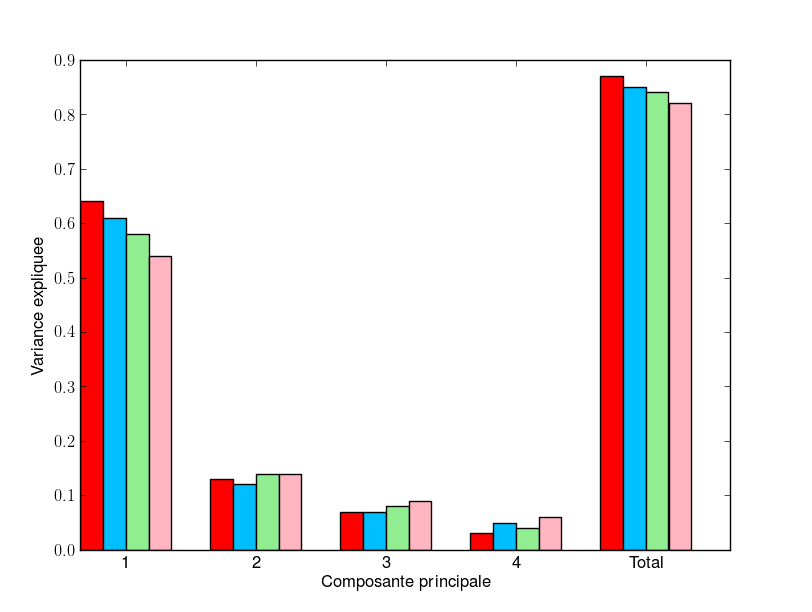
\includegraphics[scale=0.5]{./img/PCA_variance.png}
	\caption[Variance expliquée par les quatre composantes principales]{Variance expliquée par les quatre composantes principales des ACP sur $V^{R}_{f}$ (rouge), $\bar{V}^{R}_{f,genre}$ (bleu), $V^{G}_{f,genre}$ (vert) et $\bar{V}^{G}_{f,genre}$ (rose).}\label{figpcavarianceexpl}
	\end{center}	
\end{figure}	
	
	Les projections des réplicons sur les deux premières composantes sont alors utilisées pour visualiser les données. Une procédure de clustering par WARD est conduite sur les quatre premières composantes des projections de $V^{R}_{f}$ et $\bar{V}^{R}_{f,genre}$. Le choix de $k$, nombre de clusters \textit{input} de l'algorithme, est effectué en fonction du critère de stabilité $\bigtriangleup^{Kl}$ (éq. \ref{eqestimstaball}) pour $k \in \{3,10,20,50,70,100,150\}$. Les clusters obtenus sont globalement stables ($\bigtriangleup^{Kl} \thickapprox 0,75$) et sont donc interprétables (Table \ref{tabresclusterrecefunc}). 

\begin{table}[H]
	\begin{center}
	\caption[Évaluation des procédures de clustering fonctionnel des réplicons]{Évaluation des procédures de clustering de $V_{f}^{R}$ et $\bar{V}_{f,genre}^{R}$.}	\label{tabresclusterrecefunc}
	\begin{tabular}{l|c|cccc}
		 & \textbf{Indice$^{a}$}  & \multicolumn{2}{l}{\textbf{ACP+WARD}}   \\
		\hline
		 &  &  &  &   \\[-0.2cm]
		Données &  & $V_{f}^{R}$  & $\bar{V}_{f,genre}^{R}$   \\
		\multirow{2}{*}{Paramètres de WARD$^{b}$} &  & \textit{k}: 50  &  \textit{k}: 20  \\
		 &  & \textit{cp}: 4 & \textit{cp}: 4  \\
		Nombre de clusters (ACP) &  & 49 & 19  \\
		Variance expliquée (ACP) &  & 87\% & 85\%  \\
		\hline
		 &  &  &  &  \\ [-0.2cm]
		\textbf{Critère de stabilité}$^{c}$ $\bigtriangleup^{Kl}$ &  & 0.80 & 0.71  \\
		\hline
		\multirow{3}{*}{\textbf{Type de réplicon}} & \textit{homogeneity} & 0.85 & 0.68  \\
	 	& \textit{completeness} & 0.30 & 0.23 \\
		& \textit{V-measure} & 0.44 & 0.35 \\
		\hline
		\multirow{3}{*}{\textbf{Phylum des chromosomes}} & \textit{homogeneity} & 0.50 & 0.44  \\
		& \textit{completeness} & 0.27 & 0.33 \\
		& \textit{V-measure} & 0.35 & 0.38 \\
		\hline
		\multirow{3}{*}{\textbf{Classe des chromosomes}} & \textit{homogeneity} & 0.47 & 0.37  \\
		& \textit{completeness} & 0.36 & 0.41  \\
		& \textit{V-measure} & 0.41 & 0.39  \\
		\hline
		\multirow{3}{*}{\textbf{Phylum des plasmides}} & \textit{homogeneity} & 0.02 & 0.02  \\
		& \textit{completeness} & 0.10 & 0.3  \\
		& \textit{V-measure} & 0.03 & 0.03  \\
		\hline
		\multirow{3}{*}{\textbf{Classe des plasmides}} & \textit{homogeneity} & 0.03 & 0.02  \\
		& \textit{completeness} & 0.25 & 0.28  \\
		& \textit{V-measure} & 0.05 & 0.03  \\	
	\end{tabular}
	\medskip
	\captionsetup{justification=justified}
	\caption*{$^{a}$ \textit{V-measure} calculée selon l'éq. \ref{eqvm}. \\ $^{b}$ $k$, nombre de clusters en \textit{input} et $cp$ nombre de composantes principales retenues pour la classification par WARD. \\$^{c}$ Critère de stabilité $\bigtriangleup^{Kl}$ calculé par l'éq. \ref{eqestimstaball}}
	\captionsetup{}	
	\end{center}
\end{table}
		

\begin{description}
\item[\textbullet] \textbf{Chromosomes, plasmides et RECE sont discriminés fonctionnellement selon les annotations de leurs protéines des STIG.} Les chromosomes et plasmides forment deux ensembles distincts (Table \ref{tabresclusterrecefunc}; Figures \ref{figpcascatterplot} et \ref{tabrecespecificfunc}), confirmant les spécificités fonctionnelles respectives de leurs STIG. 
\end{description}
\iffalse
\begin{landscape} 
	\thispagestyle{empty}
	\begin{figure}
	\vspace{-3.5cm}
	\begin{flushleft}
	\hspace{-2cm}
	\begin{subfigure}[t]{0.42\textwidth}
	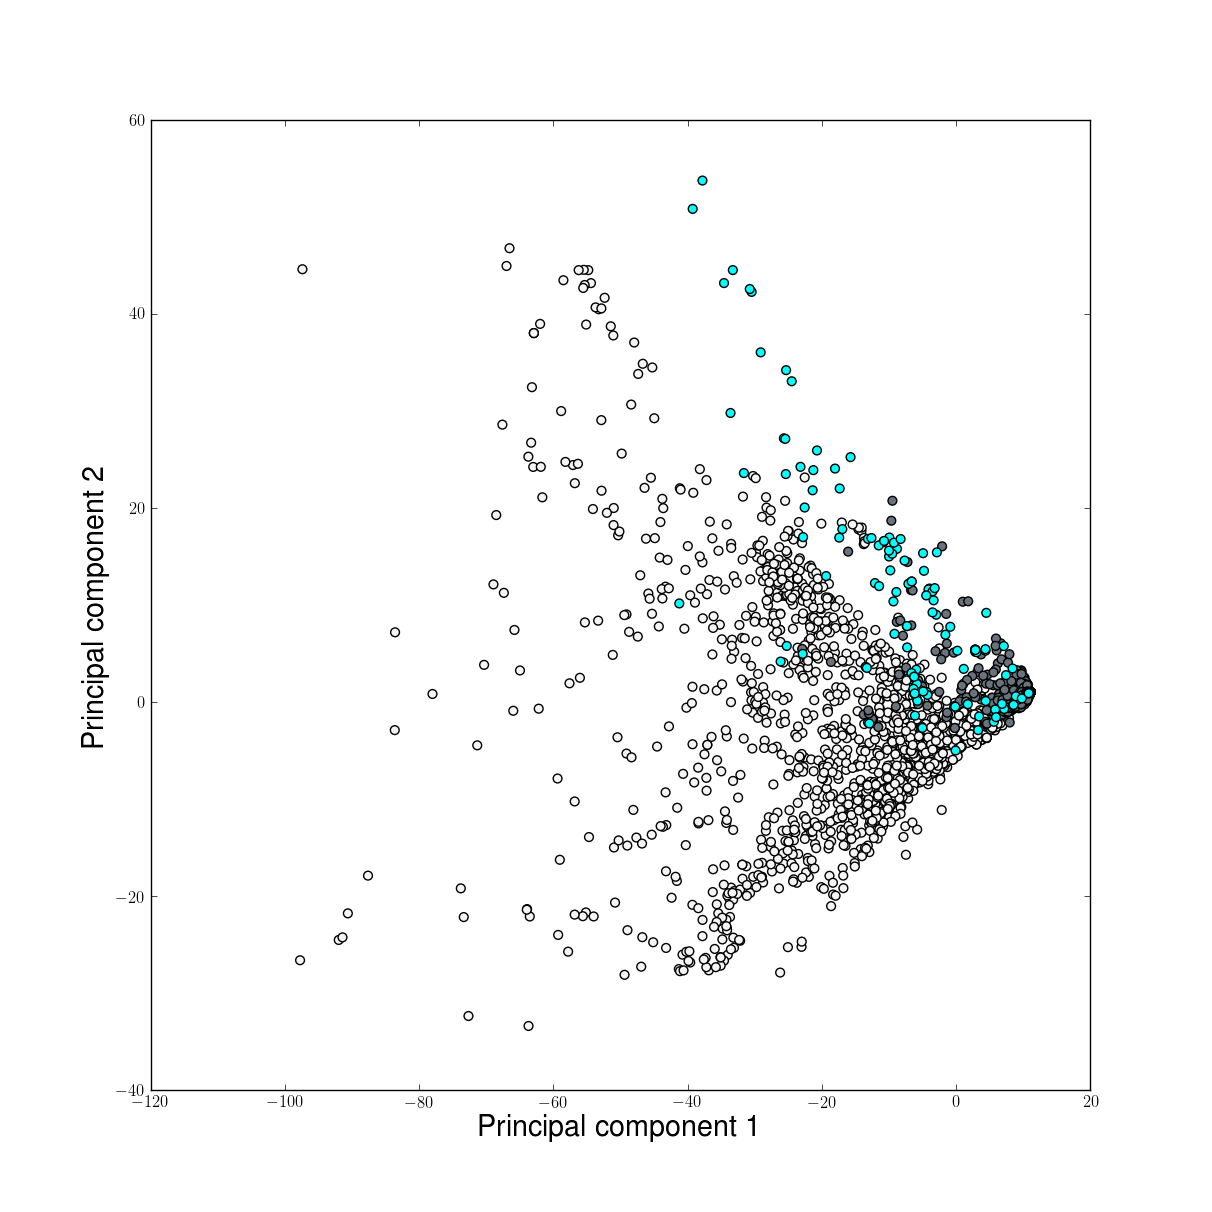
\includegraphics[width=1\textwidth]{./img/PCAcoor01.png}
	\end{subfigure}
	\begin{subfigure}[t]{0.42\textwidth}
	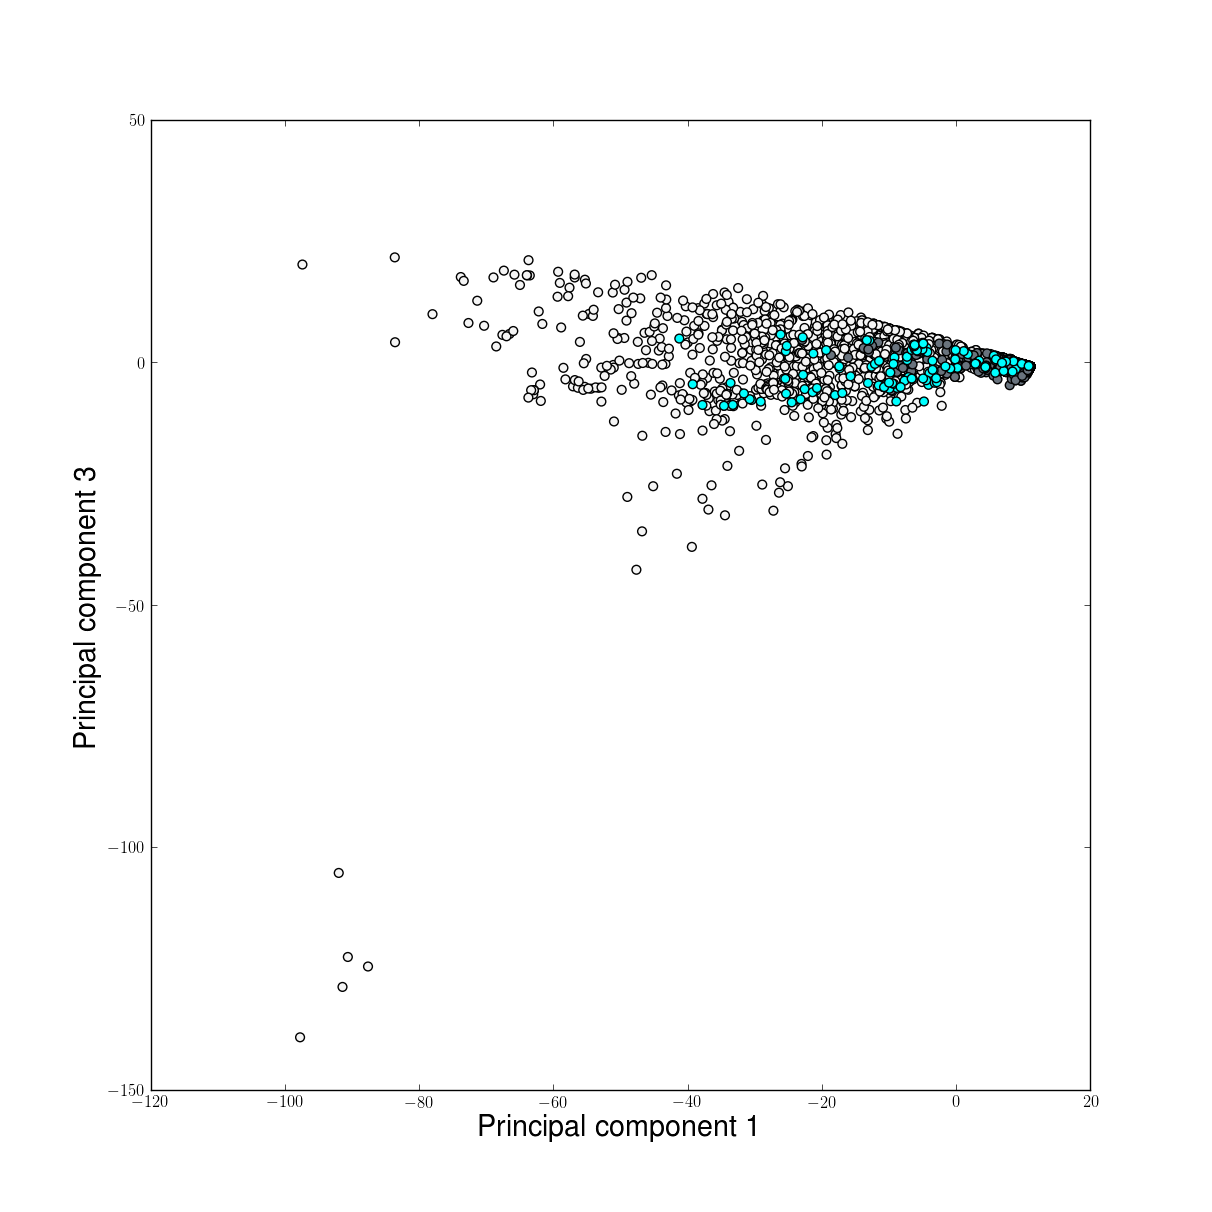
\includegraphics[width=1\textwidth]{./img/PCAcoor02.png}
	\end{subfigure}
	\begin{subfigure}[t]{0.42\textwidth}
	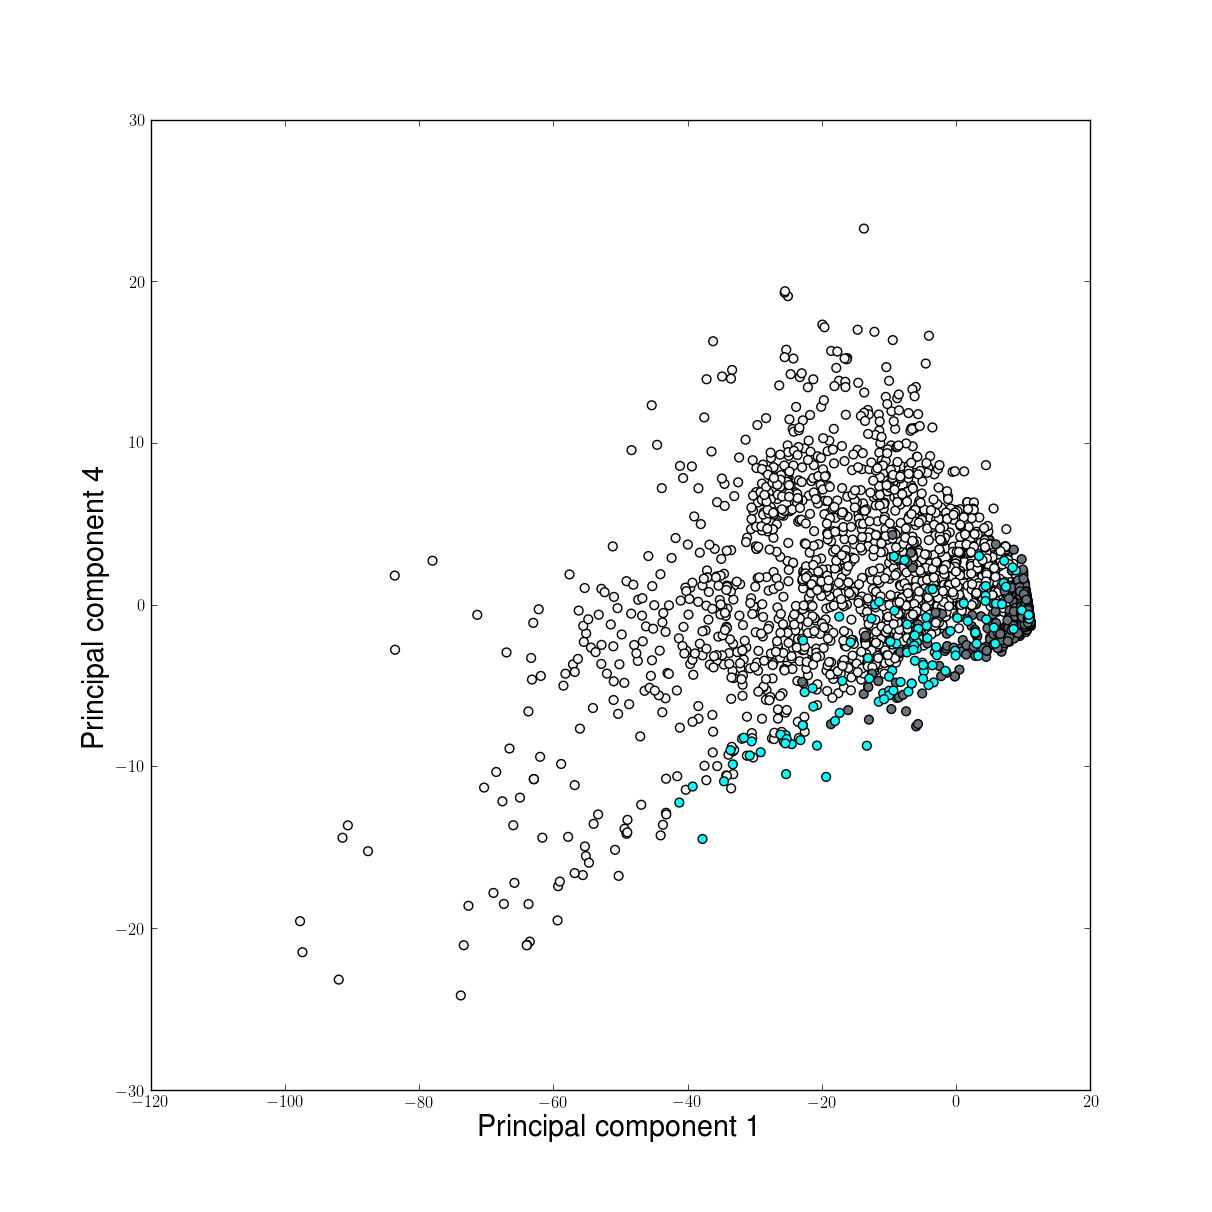
\includegraphics[width=1\textwidth]{./img/PCAcoor03.png}
	\end{subfigure}
	%\hspace{0.8cm}
	\begin{subfigure}[t]{0.42\textwidth}
	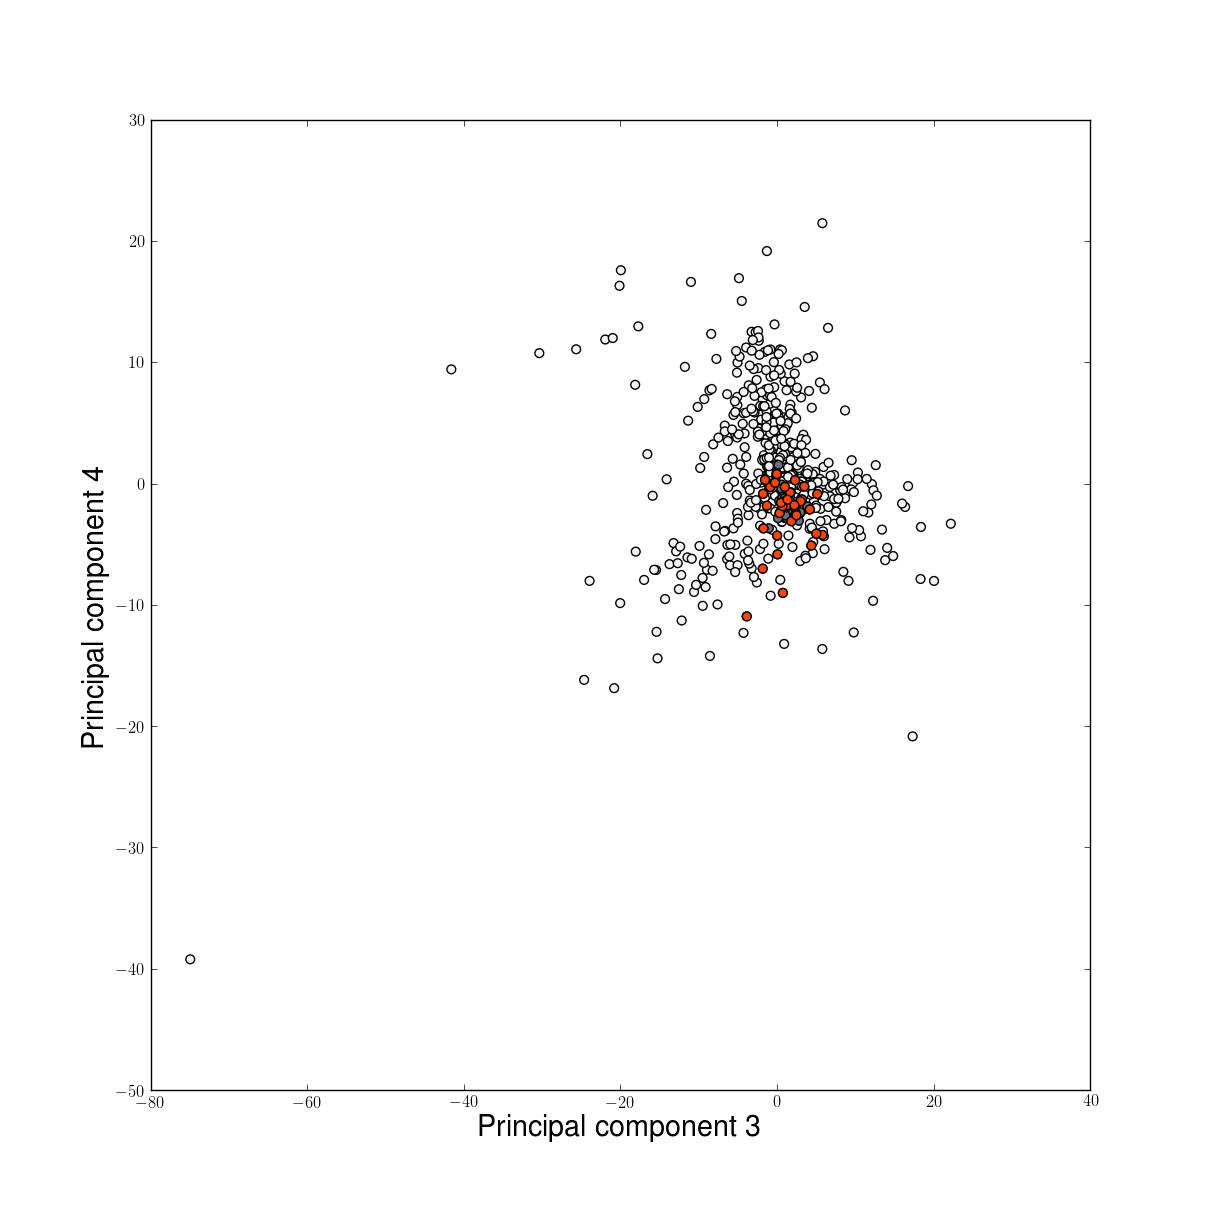
\includegraphics[width=1\textwidth]{./img/PCAncoor23.png}
	%\line(0,1){0.9\textwidth}
	\end{subfigure}
	\\
	%\vspace{-0.5cm}
	\hspace{-2cm}
	\begin{subfigure}[t]{0.42\textwidth}
	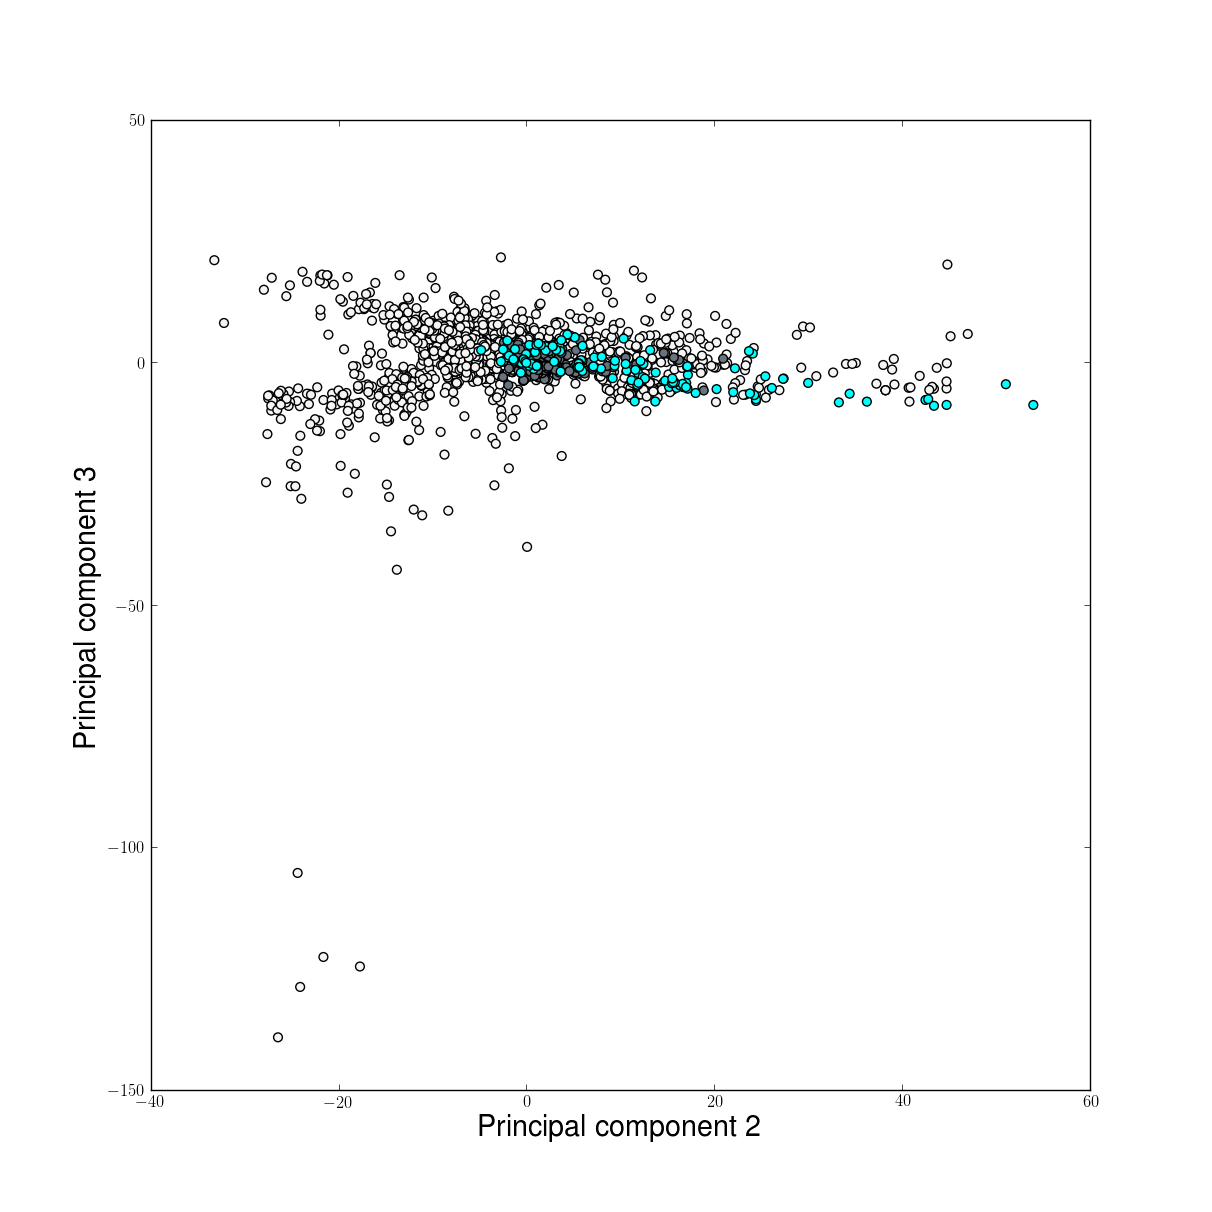
\includegraphics[width=1\textwidth]{./img/PCAcoor12.png}
	\end{subfigure}
	\begin{subfigure}[t]{0.42\textwidth}
	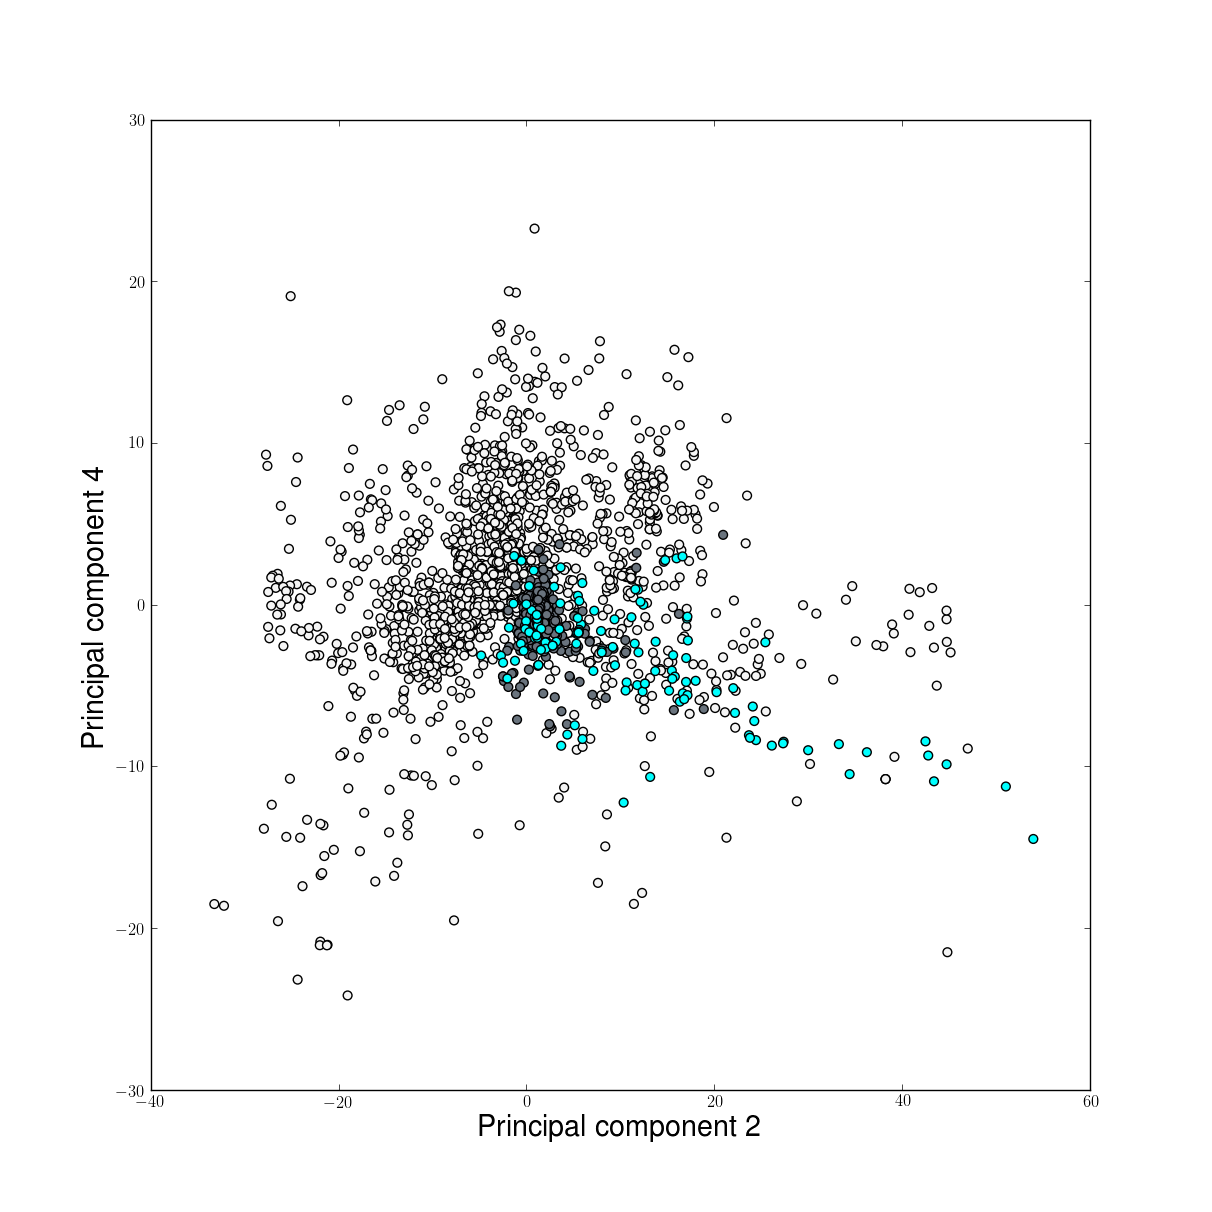
\includegraphics[width=1\textwidth]{./img/PCAcoor13.png}
	\end{subfigure}
	%\hspace{0.8cm}
	\begin{subfigure}[t]{0.42\textwidth}
	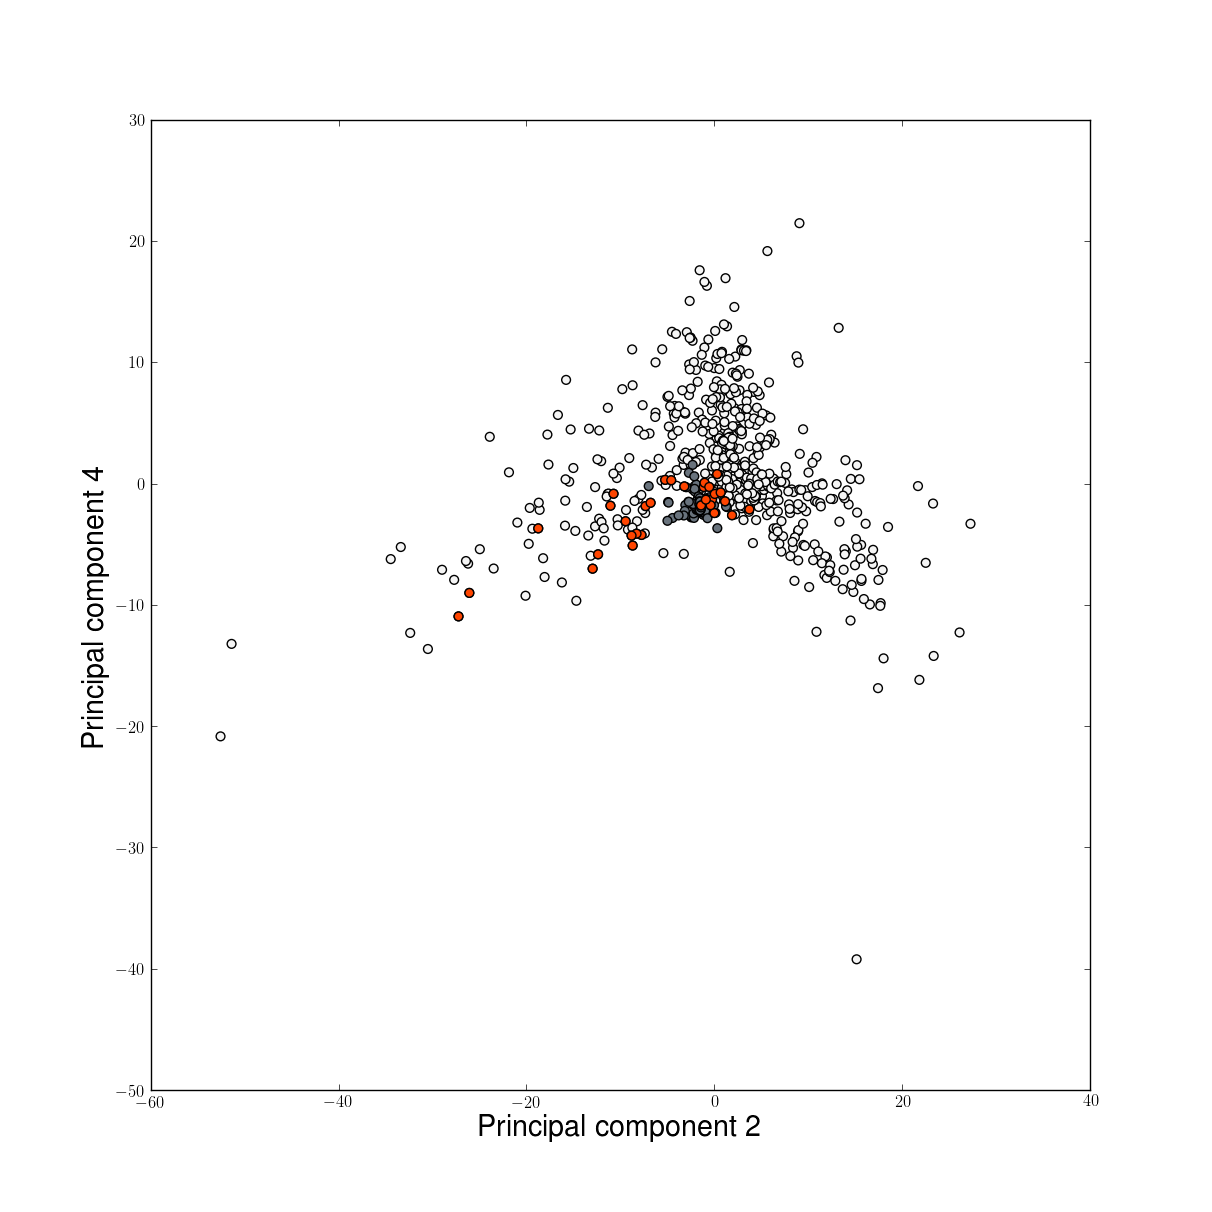
\includegraphics[width=1\textwidth]{./img/PCAncoor13.png}
	\end{subfigure}
	\begin{subfigure}[t]{0.42\textwidth}
	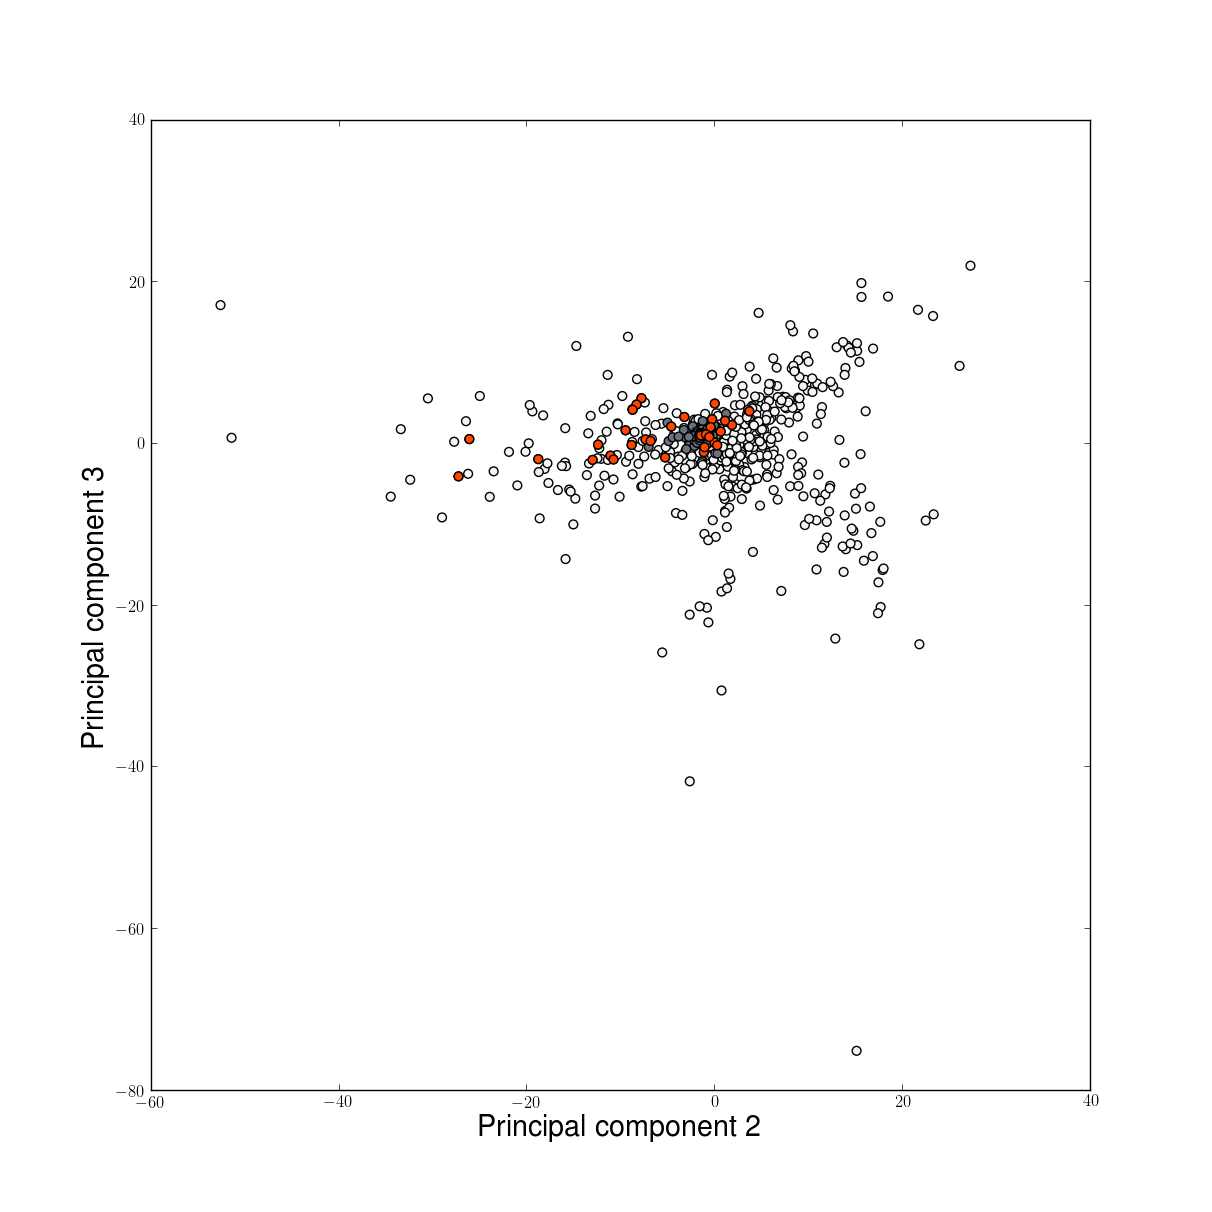
\includegraphics[width=1\textwidth]{./img/PCAncoor12.png}
	\end{subfigure}
	\\
	%\vspace{-0.5cm}
	\hspace{-2cm}
	\begin{subfigure}[t]{0.42\textwidth}
	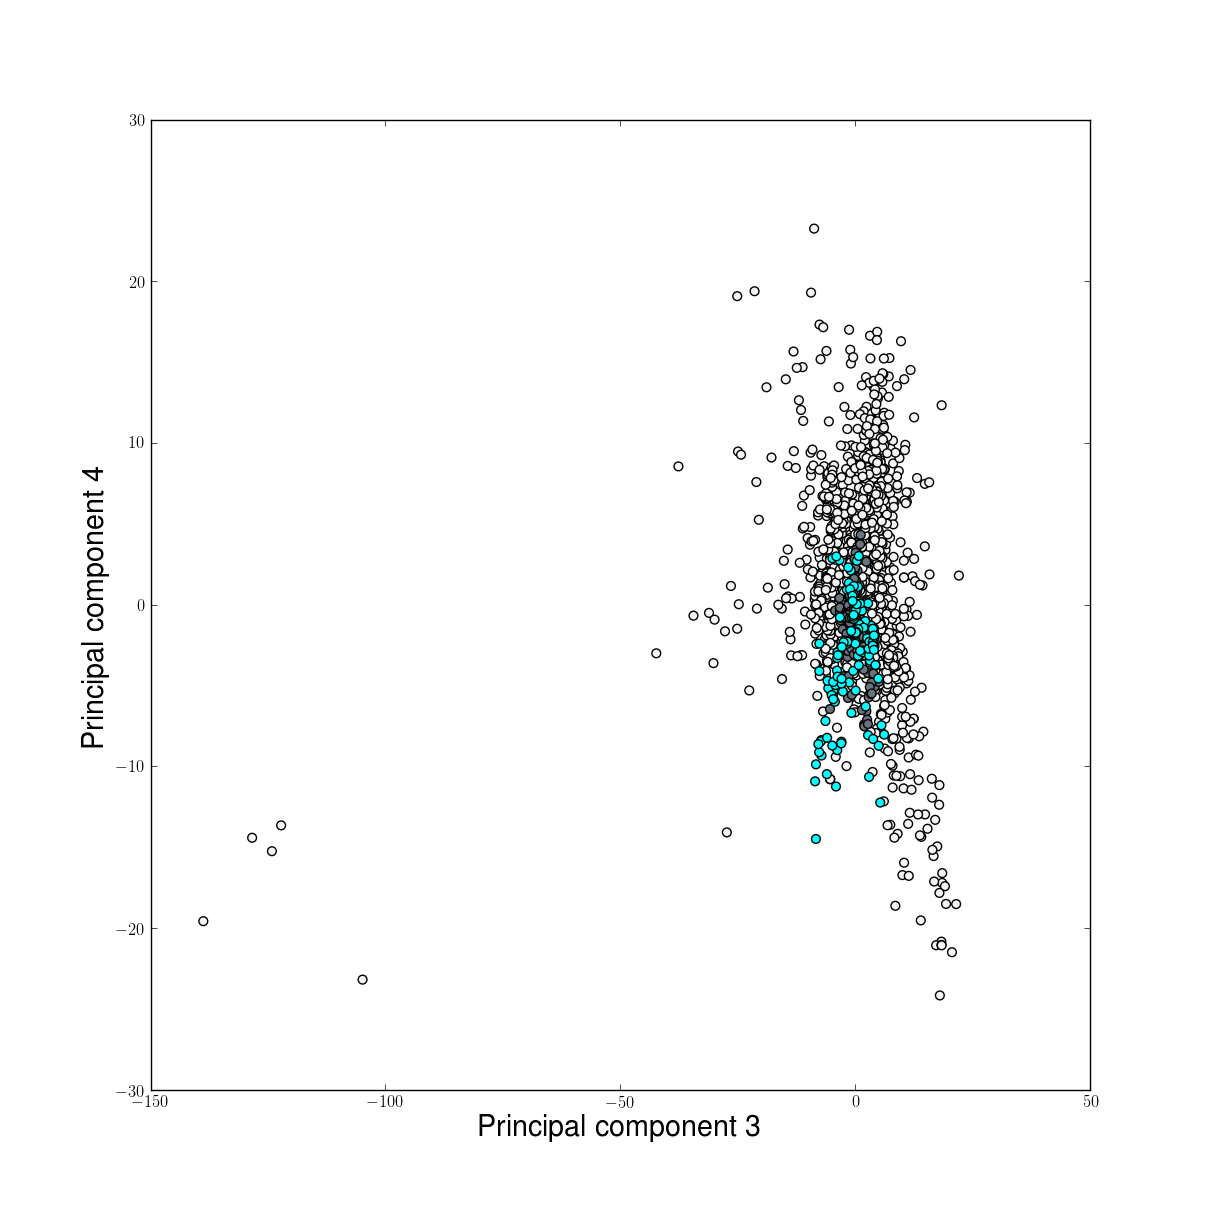
\includegraphics[width=1\textwidth]{./img/PCAcoor23.png}
	\end{subfigure}
	%\hspace{0.8cm}
	\begin{subfigure}[t]{0.42\textwidth}
	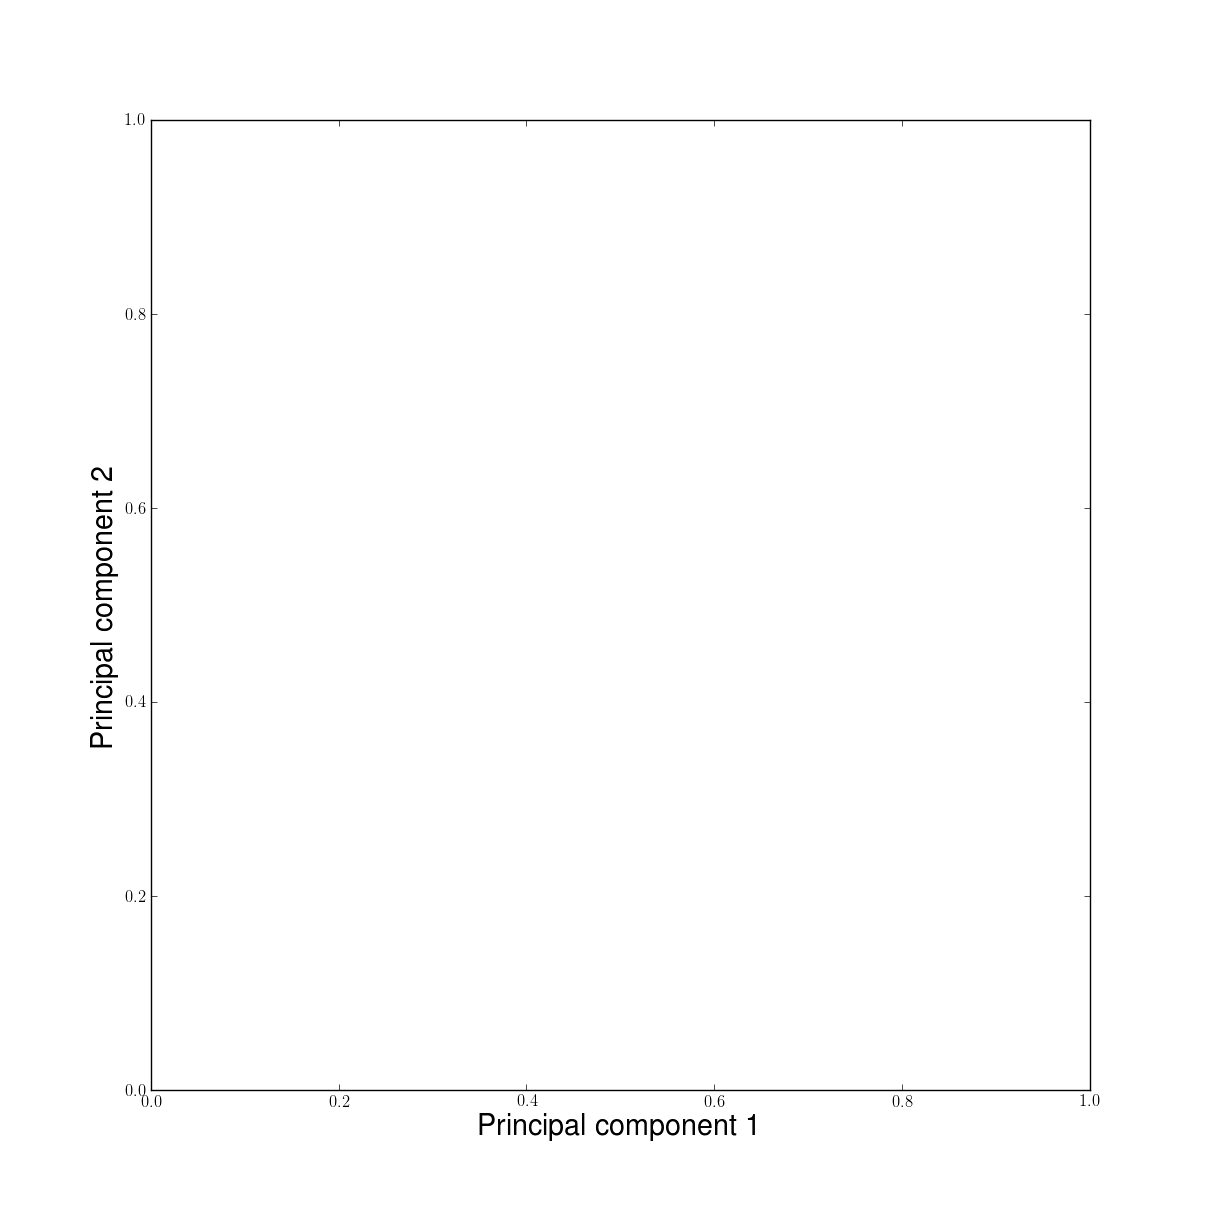
\includegraphics[width=1\textwidth]{./img/PCAncoor01.png}
	\end{subfigure}
	\begin{subfigure}[t]{0.42\textwidth}
	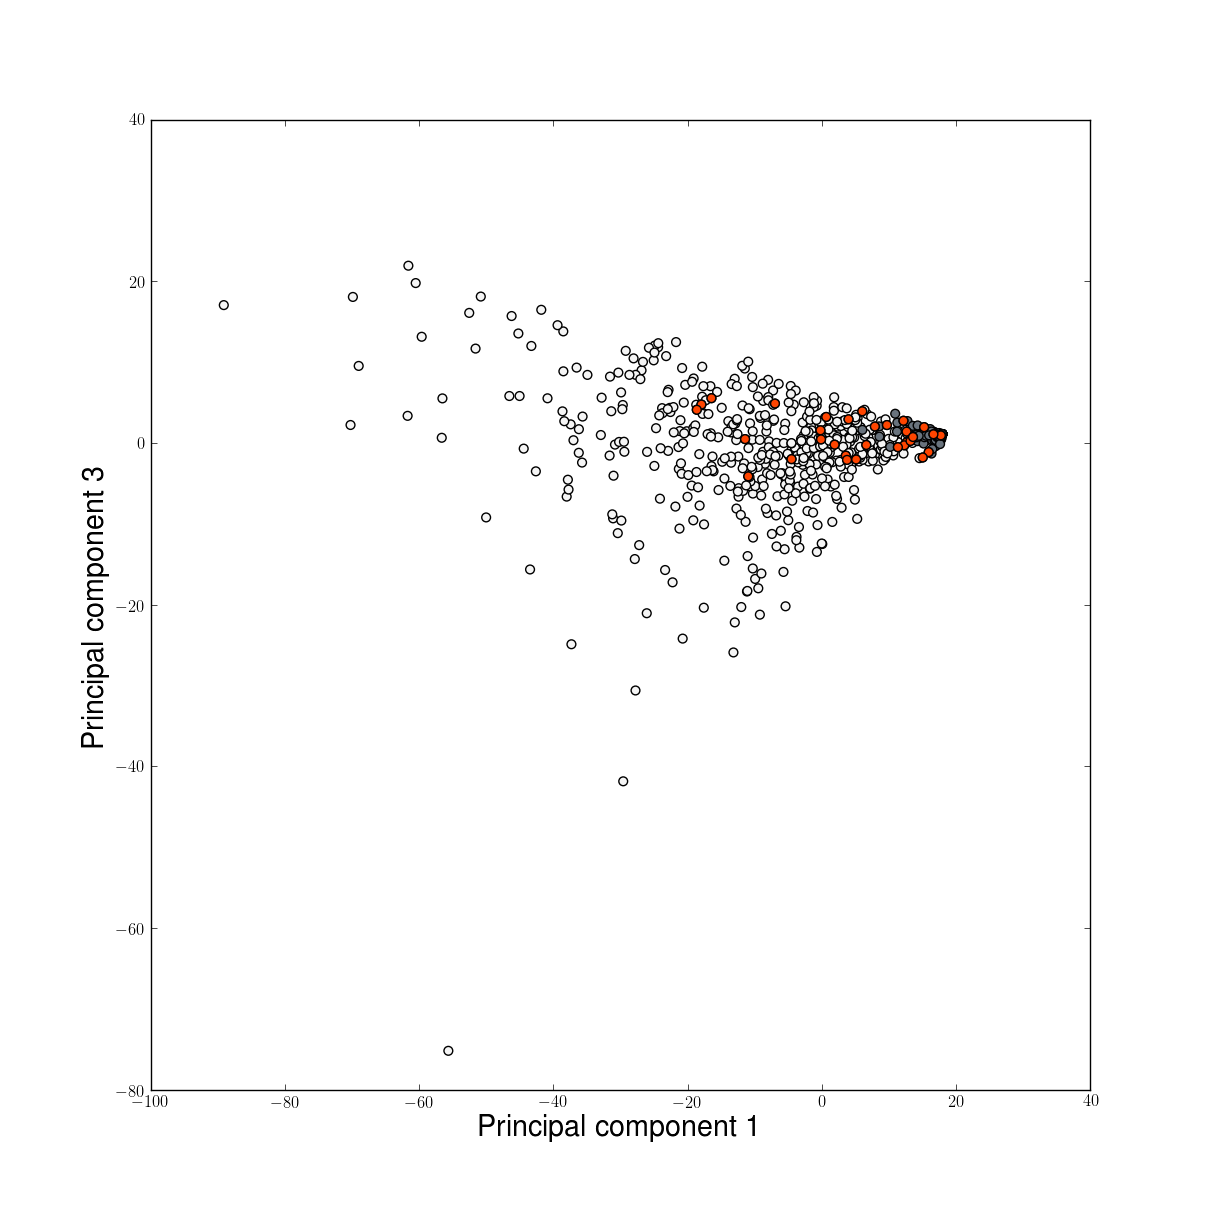
\includegraphics[width=1\textwidth]{./img/PCAncoor02.png}
	\end{subfigure}
	\begin{subfigure}[t]{0.42\textwidth}
	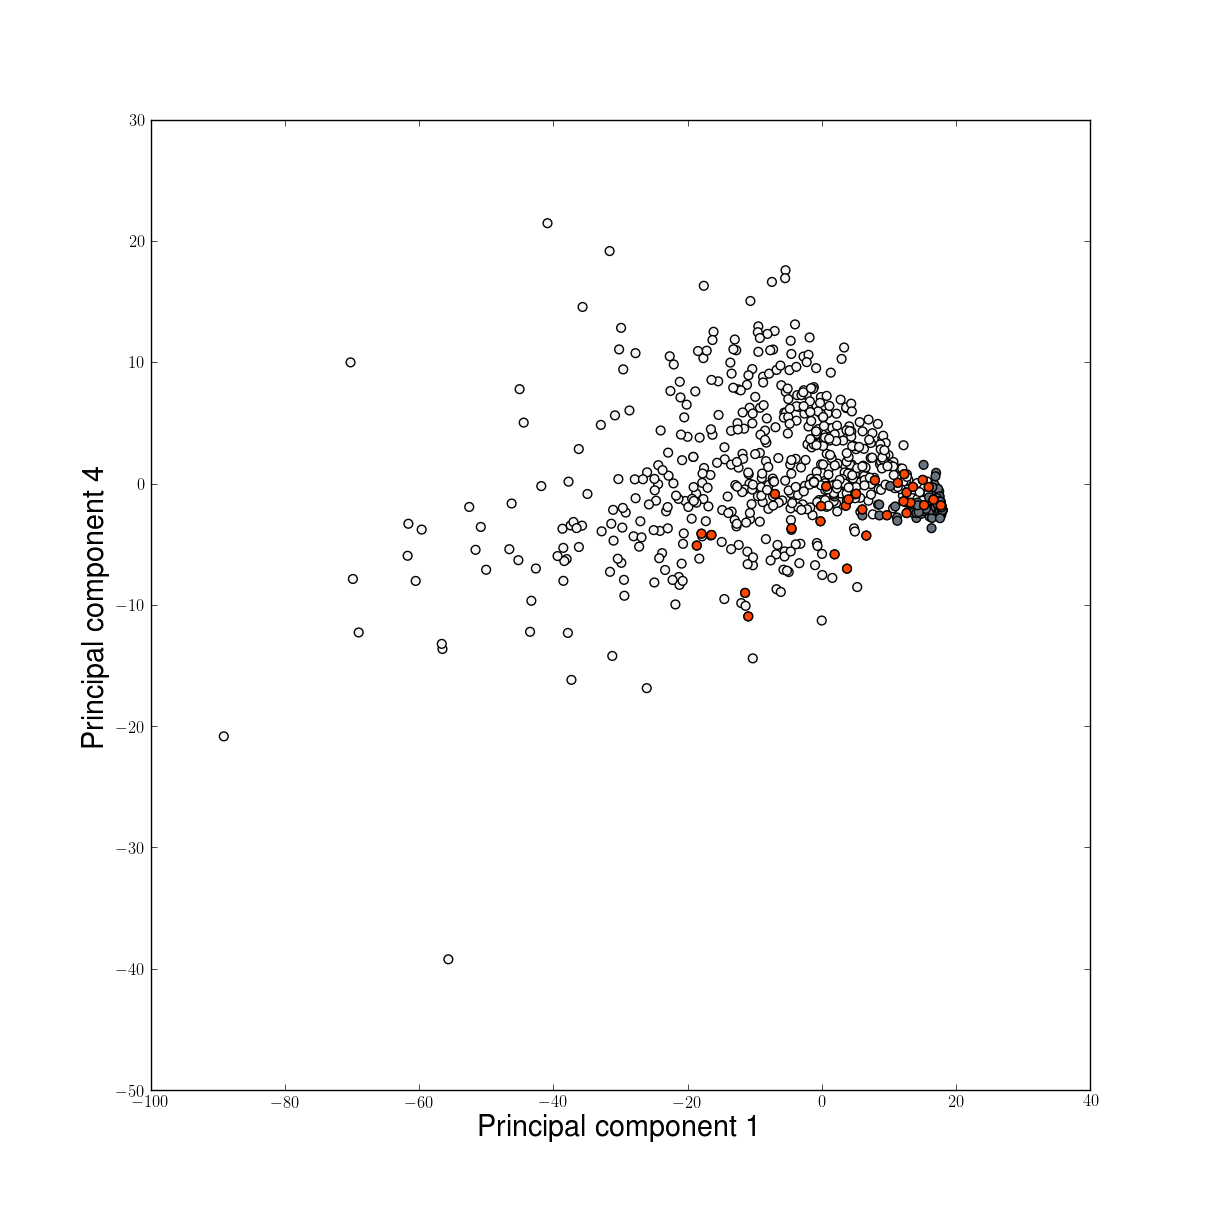
\includegraphics[width=1\textwidth]{./img/PCAncoor03.png}
	\end{subfigure}
	%\vspace{-0.5cm}
	\caption[Projection fonctionnelle des réplicons selon les quatres composantes principales de l'ACP]{Projection fonctionnelle des réplicons selon les quatre premières composantes de l'ACP sur $V^{R}_{f}$ ou $V^{R}_{f}$.\\
	Chromosome : gris clair. Plasmide : gris foncé. RECE : bleu ($V^{R}_{f}$) ou rouge ($\bar{V}^{R}_{f}$).}
	\end{flushleft}
	\end{figure}
\end{landscape}
  
\fi

\newpage
\thispagestyle{empty}
\begin{figure}[H]
\vspace{-1cm}
\hspace{-2.8cm}
	\begin{minipage}{\textwidth}
	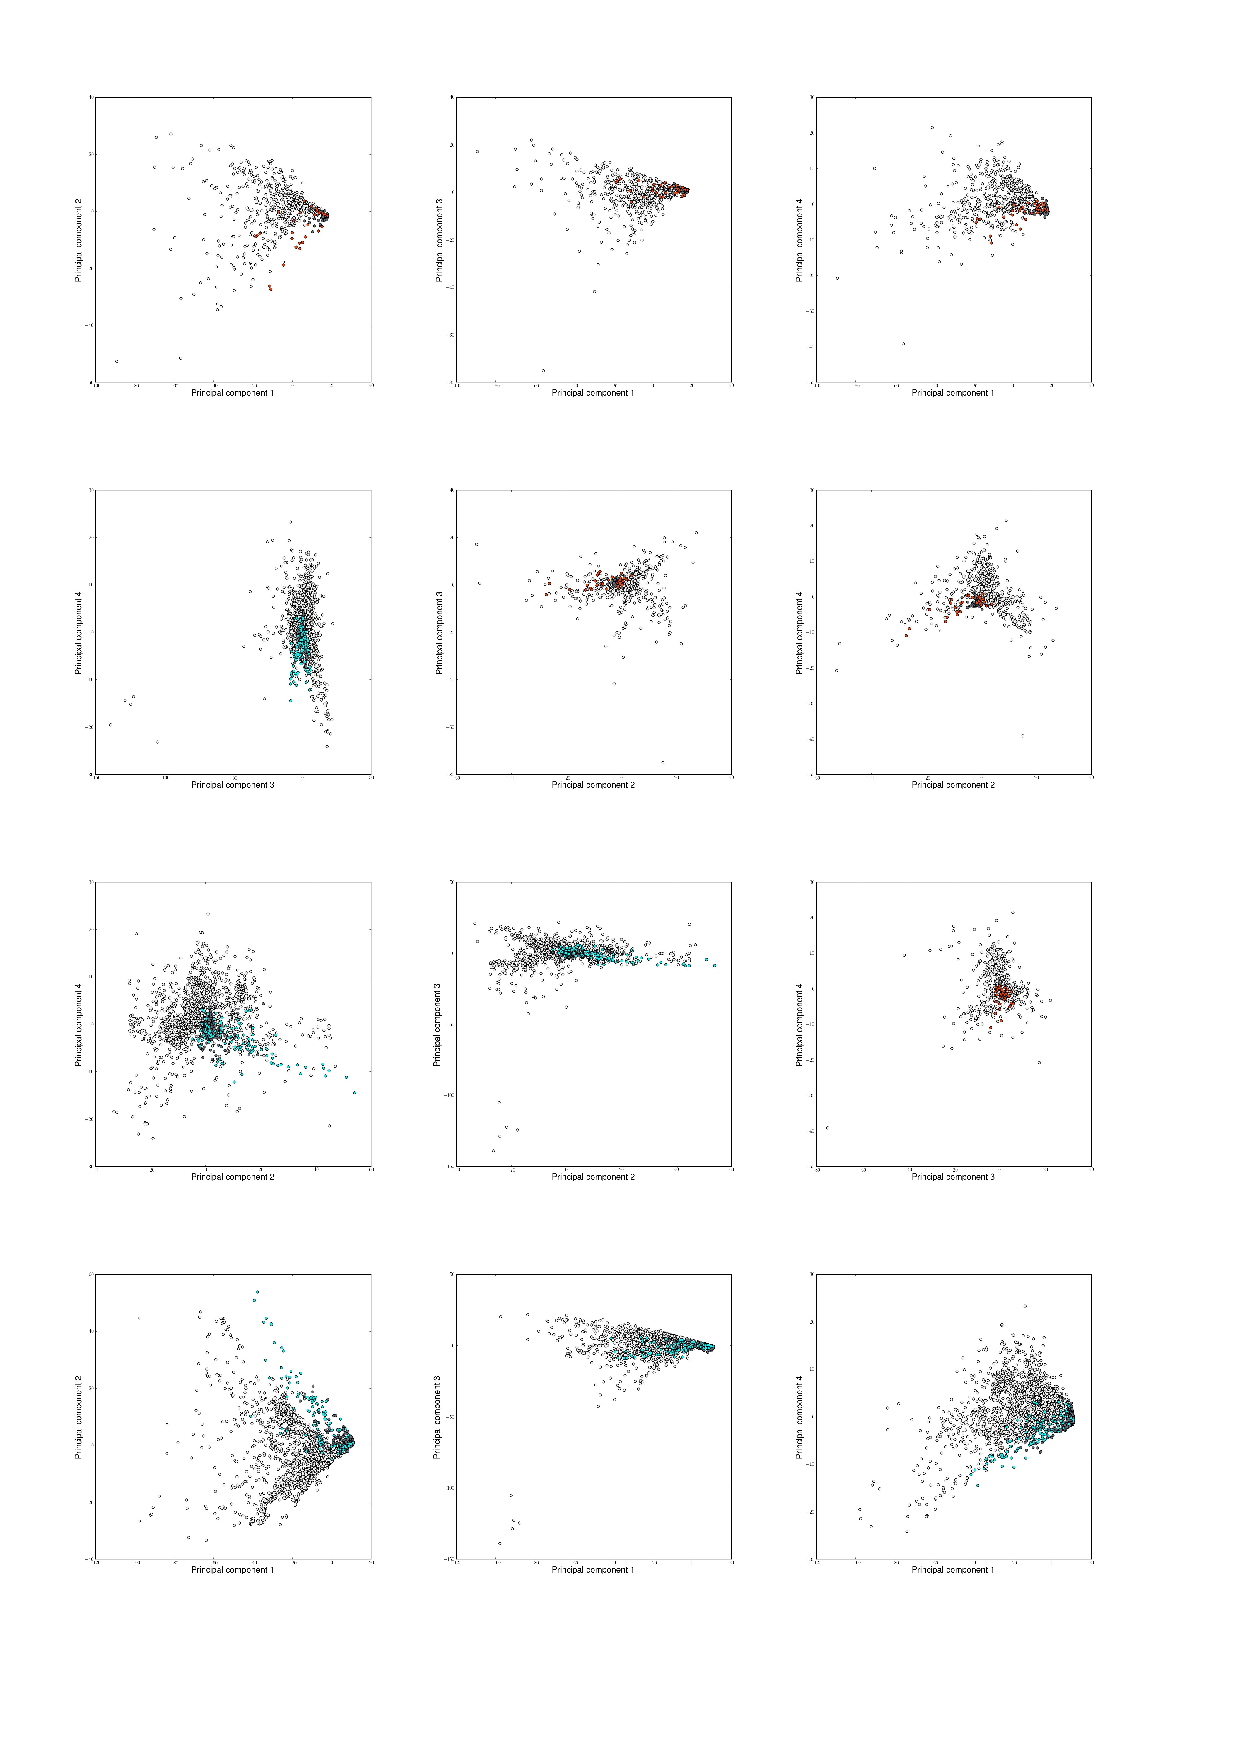
\includegraphics[trim= 0cm 2cm 0cm 0cm,clip, width=1.3\textwidth]{./img/PCA_4comp.pdf}
	\end{minipage}
\caption[Projections des réplicons selon les quatres composantes principales d'une ACP]{Projection des réplicons selon les quatre premières composantes de l'ACP sur $V^{R}_{f}$ ou $V^{R}_{f}$.\\
Chromosome : gris clair. Plasmide : gris foncé. RECE : bleu ($V^{R}_{f}$) ou rouge ($\bar{V}^{R}_{f}$).}\label{figpcascatterplot}
\end{figure}

\newpage
\begin{description}
\item[\textbullet] Les plasmides s'organisent en un groupe compact alors que différents sous-ensembles de chromosomes peuvent être identifiés (Figure \ref{figpcaproj}). Le regroupement des plasmides peut s'expliquer comme précédemment (Chapitre \ref{chap4b}), où les distances inter-plasmides sont faibles à cause du petit nombre de fonctions présentes chez eux.
\end{description}

\begin{figure}[H]
	\begin{minipage}{0.55\textwidth}
		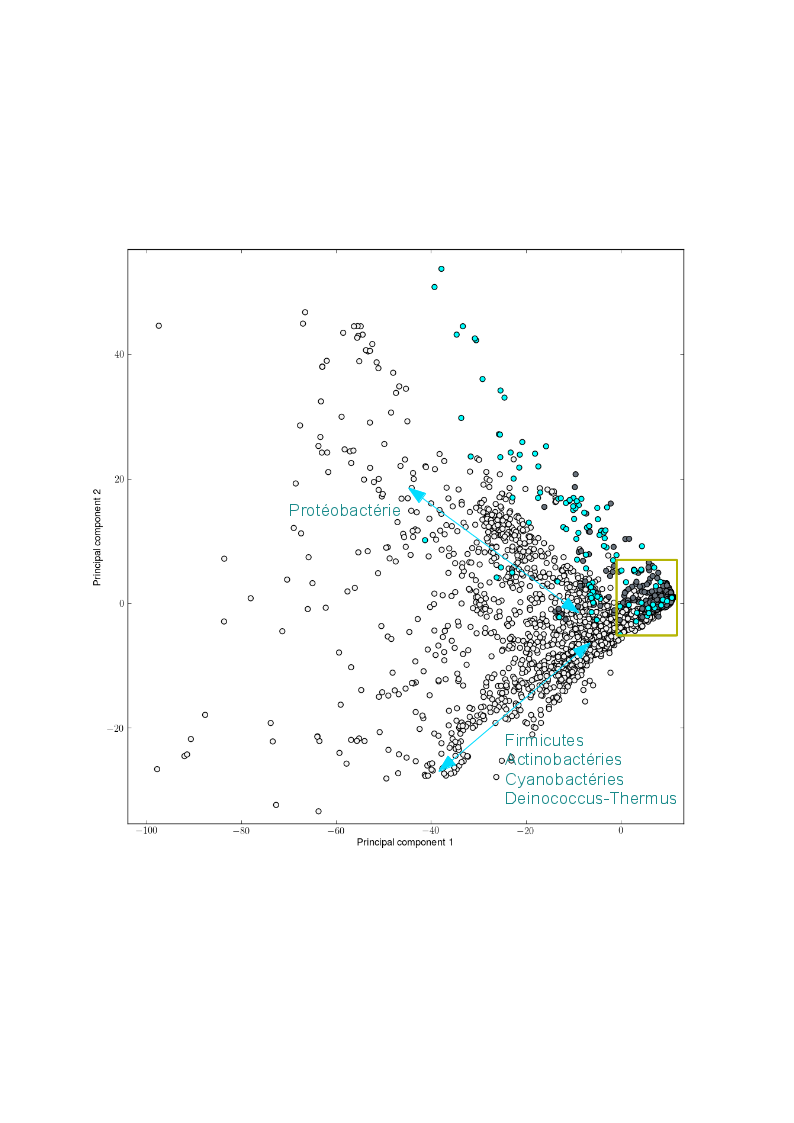
\includegraphics[trim=2cm 7cm 2cm 6cm,clip, width=\textwidth]{./img/pca_func.png}
		\subcaption{$V^{R}_{f}$}\label{figpcavr}
	\end{minipage}
	\begin{minipage}{0.55\textwidth}
		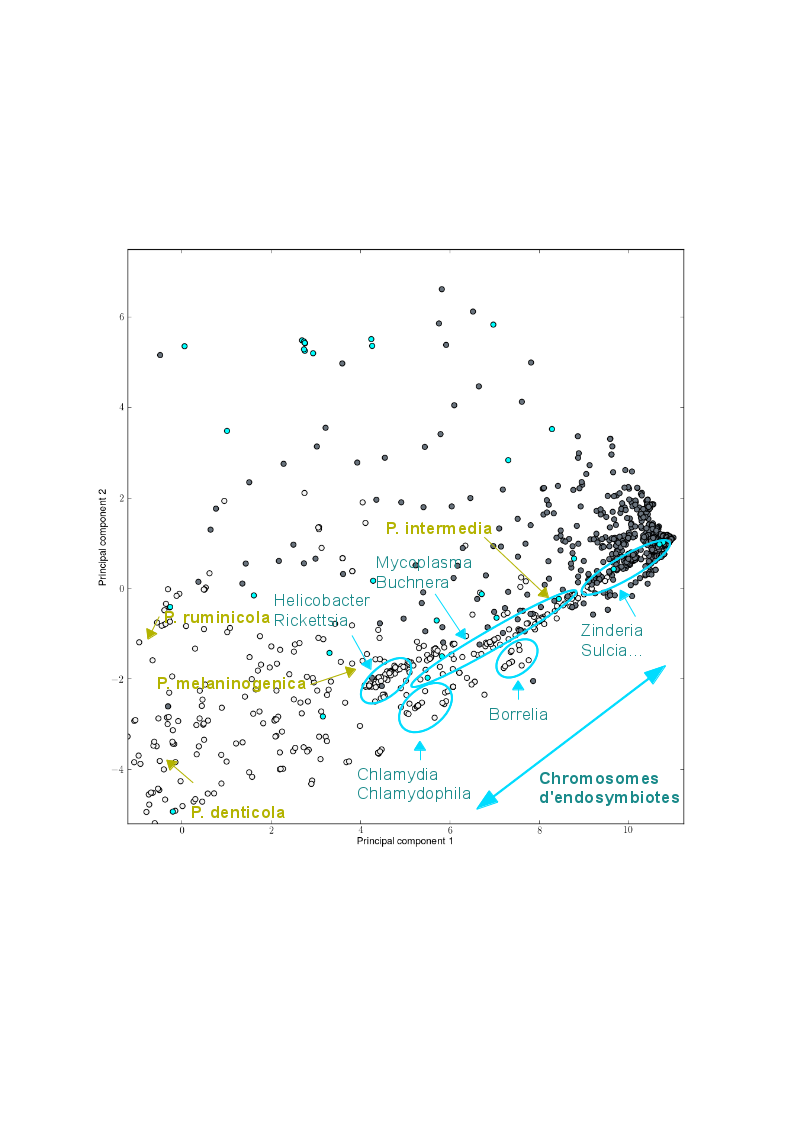
\includegraphics[trim=2cm 7cm 2cm 6cm,clip,width=\textwidth]{./img/pca_func_ZOOM.png}
		\subcaption{ZOOM}\label{figpcavrzoom}
	\end{minipage}
	\begin{minipage}{0.55\textwidth}
		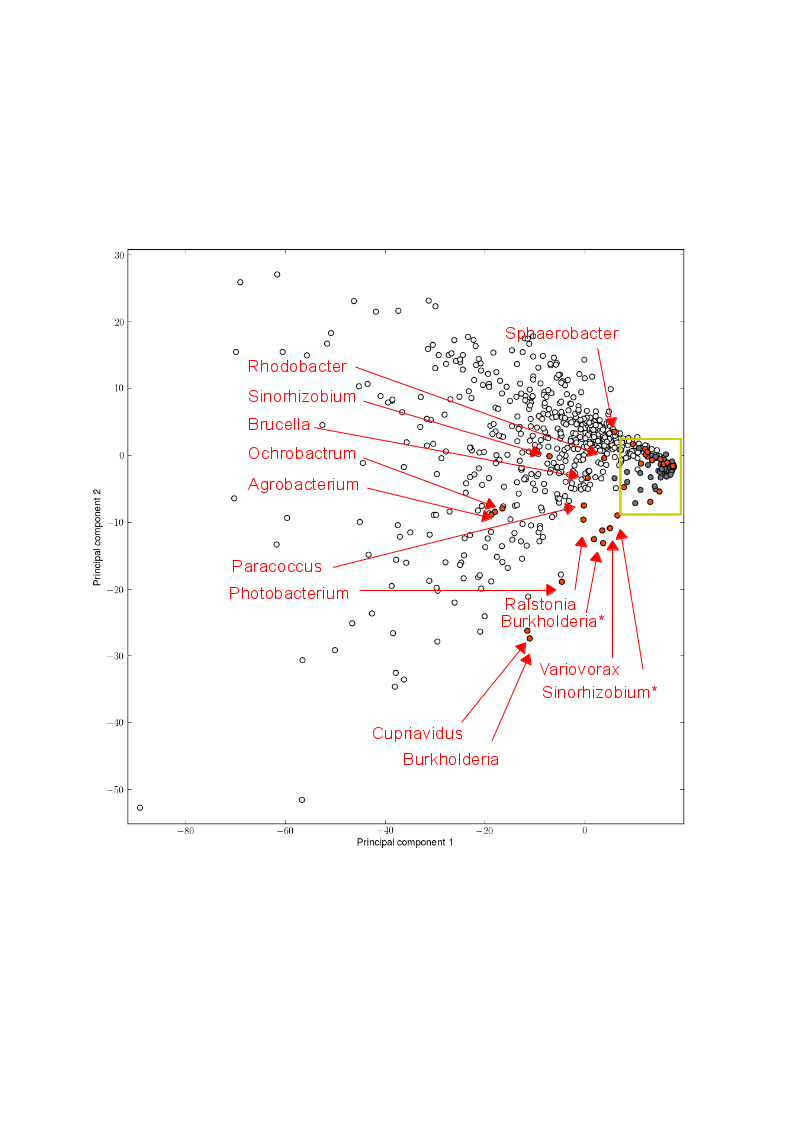
\includegraphics[trim=2cm 7cm 2cm 6cm,clip, width=\textwidth]{./img/pca_norm_func.png}
		\subcaption{$\bar{V}^{R}_{f,genre}$}\label{figpcavrnorm}
	\end{minipage}
	\begin{minipage}{0.55\textwidth}
		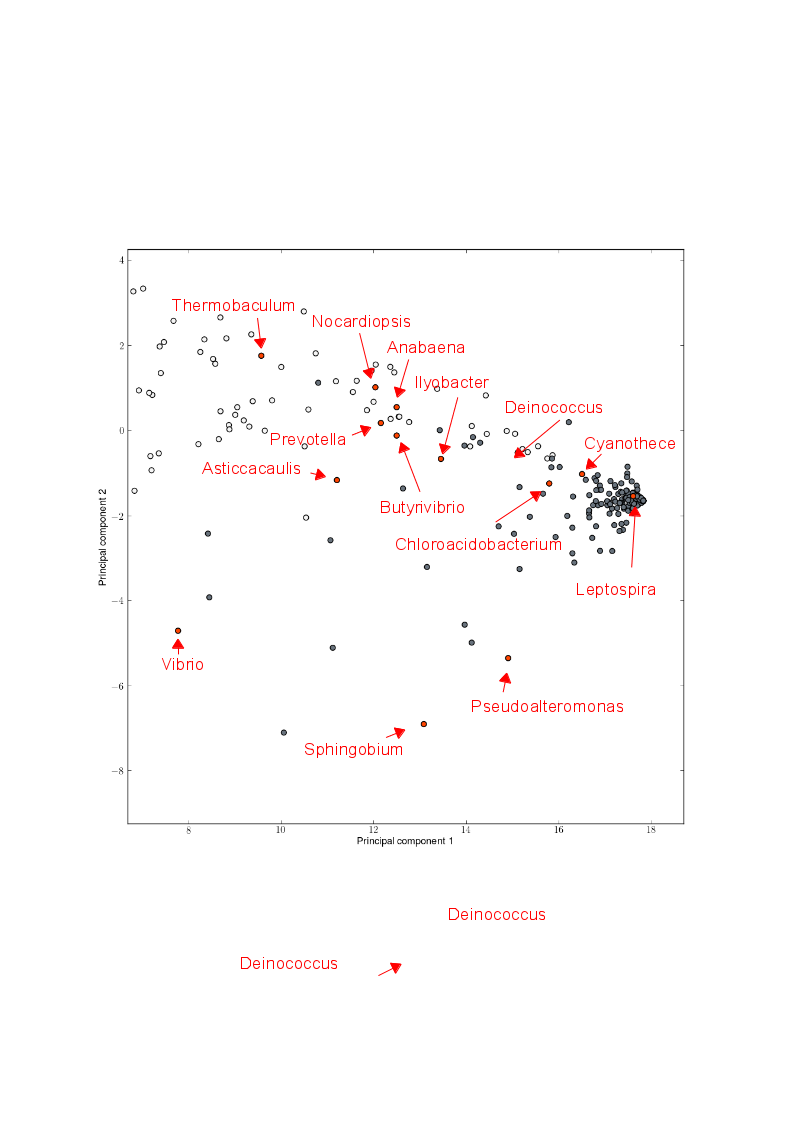
\includegraphics[trim=2cm 7cm 2cm 6cm,clip,width=\textwidth]{./img/pca_norm_func_ZOOM.png}
		\subcaption{ZOOM}\label{figpcavrnormzoom}
	\end{minipage}
	\begin{center}
	\caption[Visualisation des lignées bactériennes sur la projection des réplicons selon les deux composantes principales d'une ACP]{Visualisation des lignées bactériennes sur la projection des réplicons selon les deux composantes principales d'une ACP sur $V^{R}_{f}$ (\ref{figpcavr} et \ref{figpcavrzoom}) et, après normalisation taxinomique, sur $\bar{V}^{R}_{f}$ (\ref{figpcavrnorm} et \ref{figpcavrnormzoom}). \ref{figpcavrzoom} et \ref{figpcavrnormzoom}: zooms (rectangle) des figures \ref{figpcavr} et \ref{figpcavrnorm}, respectivement. Chromosome : gris clair. Plasmide : gris foncé. RECE : bleu ($V^{R}_{f}$) ou rouge ($\bar{V}^{R}_{f}$).} 
	\label{figpcaproj}
	\end{center}
\end{figure}	

\begin{description}
\item[\textbullet] Le nombre de variables positives dans un vecteur de réplicon n'est pas le seul facteur expliquant la discrimination des réplicons. En particulier, des RECE liés à peu de fonctions (tels que ceux d'\textit{Anabaena}, \textit{Butyrivibrio} ou \textit{Ilyobacter}) sont très nettement séparés des plasmides présentant un nombre de fonctions similaires (Figure ref{figpcavrnormzoom}). Plus généralement, les RECE se différencient des plasmides et se placent de façon caractéristique par rapport aux chromosomes (Figure \ref{tabresclusterrecefunc}), à l'exception des RECE des Spirochètes (\textit{Leptospira}; Figure ref{figpcavrnormzoom}). \textbf{\color{orange} Les RECE possèdent ainsi des spécificités fonctionnelles des STIG caractéristiques, les différenciant d'une part des chromosomes et d'autre part des plasmides}. 

\item[\textbullet]Les génomes de \textit{Prevotella} présentent un cas singulier où les chromosomes des espèces à génome multipartite \textit{(P. intermedia} et \textit{P. melaninogenica}) se distinguent de ceux des espèces à génome monopartite (\textit{P. ruminicola} et \textit{P. denticola}) en se rapprochant du groupement compact des plasmides (Figure \ref{figpcavrzoom}).

\item[\textbullet] \textbf{Sur la base de leur distribution de protéines des STIG, plusieurs types de RECE peuvent être caractérisés.} Différents niveaux de spécificité semblent exister chez les RECE, les rapprochant soit des chromosomes, soit des plasmides (Table \ref{tabresclusterrecefunc} et Figure \ref{tabrecespecificfunc}). Par exemple, les RECE des Alpha-protéobactéries semblent plus proches des chromosomes que ceux de la cyanobactérie \textit{Cyanothece} et de \textit{Candidatus} Chloroacidobacterium thermophilum (Chlorobi) qui se localisent à proximité des plasmides. Plus généralement, les résultats de ces analyses sont globalement cohérents avec les conclusions de l'étude de la totalité des réplicons (Table \ref{tabrececluster}). Les RECE ``proches" des chromosomes se retrouvent dans des clusters de chromosomes et, de même, les RECE avoisinant des plasmides (celui de \textit{Butyrivibrio} excepté) sont retrouvés dans les clusters de plasmides (Table \ref{tabrecespecificfunc}).

\item[\textbullet] \textbf{Le mode de vie des organismes bactériens influe sur les STIG de leurs réplicons génomiques.} Outre les spécificités observables de certains groupes de chromosomes de Protéobactéries, Firmicutes, Actinobactéries...(Figure \ref{figpcavr}), certains chromosomes présentent un biais de positionnement par rapport à la majorité des chromosomes et se placent à proximité des plasmides en se regroupant à leur voisinage ou avec ces derniers dans des clusters communs. Ces chromosomes appartiennent à des lignées diverses d'espèces endosymbiotiques ou de parasites/pathogènes d'eucaryotes (\textit{Rickettsia, Wolbachia, Helicobacter, Chlamydia, Mycoplasma, Borrelia, ...}). La plupart ont des tailles relativement réduites ($ \backsimeq 1 Mb$: \textit{Chlamydia}, \textit{Borrelia}...), voire très réduites ($<0.5 Mb$: \textit{Candidatus} Carsonella, \textit{Candidatus} Tremblaya...). {\bfseries \color{orange}Les génomes réduits, en adoptant une taille restreinte afin d'optimiser leur développement au sein de l'organisme hébergeant la bactérie et en relation avec la dynamique de population de la bactérie-hôte (diminution de $N_e$), développent des STIG spécifiques}. La taille n'est toutefois pas le seul facteur expliquant cette proximité. Par exemple, les génomes d'\textit{Helicobacter} (epsilon-protéobactéries) possèdent une taille relativement importante dans le contexte des génomes réduits ($\backsimeq 1.6 Mb$) mais sont fortement discriminés en comparaison à des génomes de taille similaire tels que \textit{Taylorella} (gamma-protéobactéries) ou \textit{Prochlorococcus} (Cyanobactéries).
\end{description} 

\begin{table}[H]
	\begin{center}
	\caption[Résultats de la classification non-supervisée des RECE]{Résultats de la classification non-supervisée des RECE par ACP+WARD sur $V^{R}_{f}$. Indices identiques à ceux de la Table \ref{tabrececluster}. Paramètres de l'analyse ACP+WARD décrits Table \ref{tabresclusterrecefunc}.} \label{tabrecespecificfunc} 
	\small
	\definecolor{Cchr}{RGB}{255,228,181}
	\definecolor{Cpl}{RGB}{220,220,250}
	\begin{tabular}{>{\bfseries\itshape}l|ccccccc}
		\textbf{\textnormal{Genre}} & \textbf{C} & \textbf{\footnotesize BHIw} & \textbf{\footnotesize\%chr} & \textbf{\footnotesize\%pl} & \textbf{\scriptsize\%RECE} & $E(\bigtriangleup^{r}) $ & $\bar{E}(\bigtriangleup^{C}) $ \\
		\hline
		\textit{Agrobacterium} & 3 & 0.86 & 65 & 15 & 21 & 0.95 & 0.60 \\
		\textit{Aliivibrio} & 1 & 1.00 & 0 & 30 & 70 & 0.80 & 0.70 \\
		\rowcolor{Cchr} \textit{Anabaena} & 1 & 0.21 & 77 & 19 & 4 & 0.68 & 0.64 \\
		\rowcolor{Cchr} \textit{Asticcacaulis} & 1 & 0.51 & 99 & 0 & 1 & 1.00 & 0.60 \\
		\textit{Brucella} & 1 & 0.75 & 43 & 25 & 32 & 0.98 & 0.80 \\
		\textit{Burkholderia} & 6 & 0.92 & 31 & 27 & 42 & 0.85 & 0.68 \\
		\rowcolor{Cpl} \textit{Butyrivibrio} & 1 & 0.21 & 77 & 19 & 04 & 0.68 & 0.64 \\
		\textit{Chloroacidobacterium} & 1 & 0.29 & 1 & 99 & 0 & 0.90 & 0.98 \\
		\textit{Cupriavidus} & 1 & 1.00 & 5 & 0 & 95 & 0.71 & 0.66 \\
		\rowcolor{Cpl} \textit{Cyanothece} & 1 & 0.29 & 1 & 99 & 0 & 0.90 & 0.98 \\
		\rowcolor{Cpl} \textit{Deinococcus} & 1 & 0.29 & 1 & 99 & 0 & 0.90 & 0.98 \\
		\textit{Ilyobacter} & 1 & 0.21 & 77 & 19 & 4 & 0.68 & 0.64 \\
		\rowcolor{Cpl} \textit{Leptospira} & 1 & 0.29 & 1 & 99 & 0 & 0.90 & 0.98 \\
		\textit{Nocardiopsis} & 1 & 0.21 & 77 & 19 & 4 & 0.68 & 0.64 \\
		\textit{Ochrobactrum} & 1 & 1.0 & 90 & 3 & 7 & 0.75 & 0.39 \\
		\rowcolor{Cchr} \textit{Paracoccus} & 1 & 0.89 & 92 & 3 & 5 & 0.53 & 0.32 \\
		\textit{Photobacterium} & 1 & 1.00 & 0 & 30 & 70 & 0.80 & 0.70 \\
		\rowcolor{Cchr} \textit{Prevotella} & 2 & 0.34 & 87 & 11 & 3 & 0.74 & 0.62 \\
		\textit{Pseudoalteromonas} & 1 & 0.21 & 77 & 19 & 4 & 0.68 & 0.64 \\
		\textit{Ralstonia} & 2 & 1.00 & 11 & 22 & 77 & 0.77 & 0.69 \\
		\rowcolor{Cpl} \textit{Rhodobacter} & 2 & 0.84 & 27 & 41 & 32 & 0.97 & 0.73 \\
		\rowcolor{Cpl} \textit{Sinorhizobium} & 2 & 0.86 & 25 & 27 & 48 & 0.87 & 0.76 \\
		\textit{Sphaerobacter} & 1 & 0.35 & 100 & 0 & 0 & 1.00 & 0.60 \\
		\rowcolor{Cpl} \textit{Sphingobium} & 2 & 34 & 64 & 27 & 9 & 0.84 & 0.64 \\
		\textit{Thermobaculum} & 1 & 0.21 & 77 & 19 & 4 & 0.68 & 0.64 \\
		\textit{Variovorax} & 1 & 1.00 & 0 & 30 & 70 & 0.80 & 0.70 \\
		\textit{Vibrio} & 4 & 0.97 & 31 & 32 & 37 & 0.83 & 0.57 \\
	\end{tabular}
	\end{center}
\end{table}	

\section{Discrimination fonctionnelle des génomes} 

	La même analyse a été appliquée aux génomes ($V_{f}^{G}$ et $\bar{V}_{f,genre}^{G}$). L'ACP a été utilisée pour projeter les données dans un espace de dimension réduite afin de les visualiser et les clusteriser. Les quatre principales composantes ont de plus été utilisées pour la classification par WARD. Le choix de $k$ pour l'analyse de clustering est fondé sur le critère de stabilité $\bigtriangleup^{Kl}$ (éq. \ref{eqestimstaball}) pour $k \in \{3,10,20,50,70,100,150\}$. 
	 
\begin{table}[H]
	\begin{center}
	\caption[Évaluation du clustering fonctionnel des génomes.]{Évaluation du clustering fonctionnel des génomes.} 	\label{tabresclustergenomefunc}
	\begin{tabular}{l|l|cccc}
		& \textbf{Indices$^{a}$}  & \multicolumn{2}{c}{\textbf{ACP+WARD}}   \\
		\hline
		& & & &  \\[-0.2cm]
		Données &  & $V_{f}^{G}$ & $\bar{V}_{f,genre}^{G}$  \\
		\multirow{2}{*}{Paramètres de WARD $^{b}$} &  & \textit{k}: 150  & \textit{k}: 70  \\
		&  & \textit{cp}: 4 & \textit{cp}: 4 \\
		Nombre de clusters ACP &  & 142 & 60 \\
		Variance expliquée ACP & & 82\% & 81\% \\
		\hline
		 & & & &  \\[-0.2cm]
		\textbf{Critère de stabilité$^{c}$} $\bigtriangleup^{Kl}$ &  & 0.68 & 0.58  \\
		\hline
		\multirow{3}{*}{\textbf{Type de génome}} & \textit{homogeneity} & 0.60 & 0.39  \\
		& \textit{completeness} & 0.03 & 0.02 \\
		& \textit{V-measure} & 0.05 & 0.04 \\
		\hline
		\multirow{3}{*}{\textbf{Phylum des génomes}} & \textit{homogeneity} & 0.51 & 0.55 \\
		& \textit{completeness} & 0.22 & 0.29 \\
		& \textit{V-measure} & 0.31 & 0.38 \\
		\hline
		\multirow{3}{*}{\textbf{Classe des génomes}} & \textit{homogeneity} & 0.51 & 0.51 \\
		& \textit{completeness} & 0.32 & 0.39 \\
		& \textit{V-measure} & 0.39 & 0.44 \\
	\end{tabular}
	\medskip
	\captionsetup{justification=justified}
	\caption*{\footnotesize {$^{a}$ \textit{V-measure} calculée selon l'éq. \ref{eqvm}. \\ $^{b}$ $k$, nombre de clusters en \textit{input} et $cp$, nombre de composantes principales retenues pour la classification par WARD. \\ $^{c}$ Critère de stabilité $\bigtriangleup^{Kl}$ calculé par l'éq. \ref{eqestimstaball}}}.
	\captionsetup{}
	\end{center}
 \end{table}

	 Les clusters de génomes obtenus par ACP+WARD sont plus instables que ceux obtenus pour les réplicons (Table \ref{tabresclustergenomefunc}) et sont donc difficilement interprétables et potentiellement fortement bruités. Les critères d'\textit{homogeneity} indiquent de plus qu'il n'y a \textit{a priori} pas de séparation nette détectable entre génomes mono- et multipartites. Cependant, les projections des données selon les quatre composantes principales de l'ACP sont pertinentes compte-tenu de la variabilité expliquée ($>80\%$, Table \ref{tabresclustergenomefunc}). De plus, les projections de $\bar{V}_{f,genre}^{G}$ montrent des tendances similaires à celles de $V_{f}^{G}$ (Figure \ref{figpcagenome}). \\
 		

\begin{figure}
	\begin{minipage}{0.55\textwidth}
		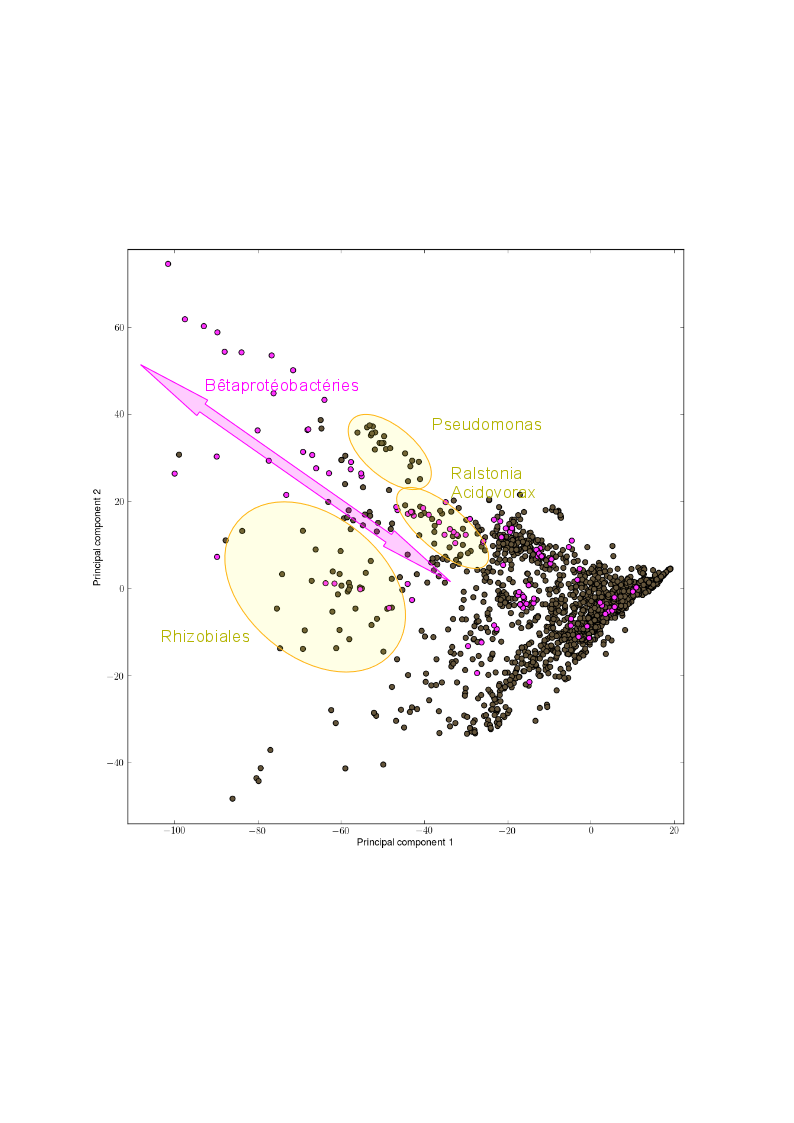
\includegraphics[trim=2cm 7cm 2cm 6cm,clip, width=\textwidth]{./img/pca_genome.png}
		\subcaption{$V^{G}_{f}$}\label{figpcavg}
	\end{minipage}
	\begin{minipage}{0.55\textwidth}
		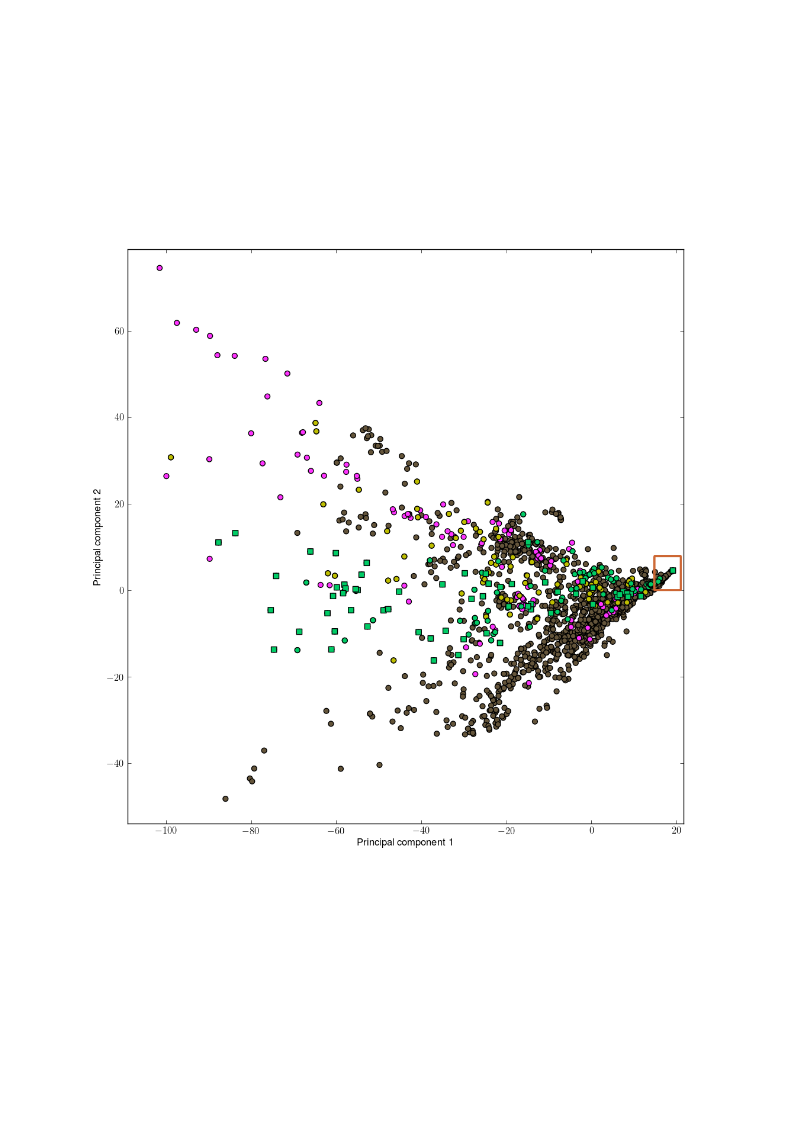
\includegraphics[trim=2cm 7cm 2cm 6cm,clip,width=\textwidth]{./img/pca_genome_II.png}
		\subcaption{$V^{G}_{f}$}\label{figpcavg2}
	\end{minipage}
	\begin{center}
	\begin{minipage}{0.55\textwidth}
		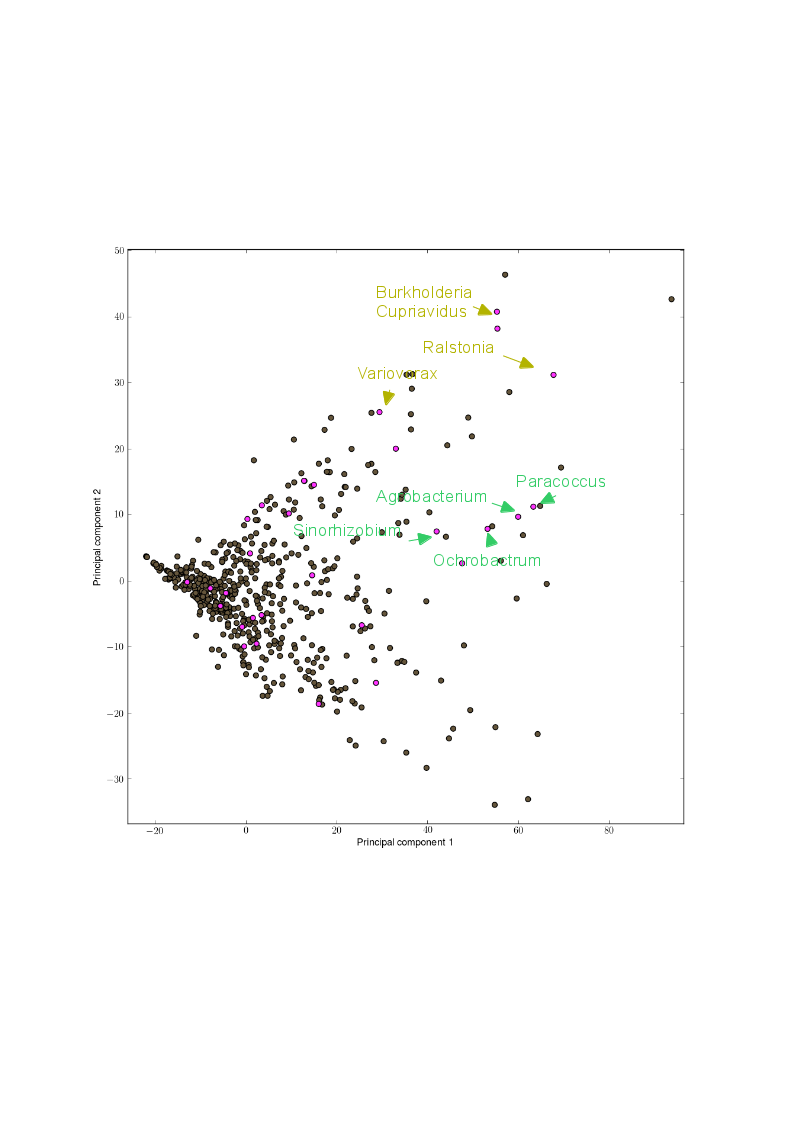
\includegraphics[trim=2cm 7cm 2cm 6cm,clip,width=\textwidth]{./img/pca_genome_norm.png}
		\subcaption{$\bar{V}^{G}_{f,genre}$}\label{figpcavg3}
	\end{minipage}
	\caption[Projection fonctionnelle des génomes selon les deux composantes principales d'une ACP ]{Projection fonctionnelle des génomes selon les deux composantes principales d'une ACP sur $V^{G}_{f}$ (A,B) ou  $\bar{V}^{G}_{f,genre}$ (C). \\ Génomes monopartites : gris foncé; génomes multipartites: magenta. Bêtaprotéobactéries: kaki, Alphaprotéobactéries: vert.\\
A: Visualisation de la tendance de répartition des Bêta-protéobactéries (rose) et de groupes majoritairement formés de génomes monopartites (jaune). B: Visualisation des localisations des génomes monopartites des Bêtaprotéobactéries et des Alphaprotéobactéries (Rhizobiales indiquées par des marqueurs carré). Rectangle rouge à droite de la figure: génomes uniquement composés de plasmides. C: Visualisation des génomes multipartites les plus différenciés parmi les Bêtaprotéobactéries (kaki) et les Alphaprotéobactéries (vert) selon une projection de $\bar{V}^{G}_{f,genre}$ sur les deux composantes principales.} \label{figpcagenome}
	\end{center}
\end{figure}
	  	

\begin{description}
	\item[\textbullet] \textbf{Aucune tendance générale ne caractérise les génomes multipartites dans leur globalité}. Les variables utilisées ne permettent pas de mettre en avant une discrimination significative des génomes multipartites par rapport aux génomes monopartites (Table \ref{tabresclustergenomefunc}). D'éventuelles spécificités des génomes qui, à l'échelle des réplicons étaient clairement visibles, sont peut-être “noyées” dans la masse des données génomiques. Alternativement, il est possible que l'on ne dispose de pas suffisamment de variables pour qu’émerge une tendance caractéristique des génomes multipartites.
	
	\item[\textbullet] \textbf{Certains génomes, dont une part importante de génomes multipartites, sont cependant clairement discriminés.} Les projections indiquent que certains génomes s'écartent de l'ensemble des génomes (Figure \ref{figpcagenome}). Ils englobent les génomes multipartites des Bêtaprotéobactéries ainsi qu'une part importante des génomes des Rhizobiales (Alphaprotéobactéries). Ces génomes appartiennent majoritairement à des espèces associées à des plantes, parmi lesquelles des pathogènes mais surtout des mutualistes qui sont connus pour échanger des gènes impliqués dans le développement de l'association symbiotique aux plantes. Au-delà des gènes impliqués dans la symbiose avec un hôte eucaryote, \textbf{\color{orange} l'écologie particulière de ces organismes (symbiotes des plantes) est corrélée à une adaptation spécifique des STIG de ces génomes}. Cette corrélation n'étant pas détectable sur les analyses des réplicons (Figure \ref{figpcaproj}), on peut proposer l'hypothèse corollaire que \textbf{\color{orange} cette adaptation des STIG passe par l'adaptation des réplicons extra-chromosomiques}. Ces hypothèses sont toutefois à considérer avec prudence, compte tenu de l'instabilité des données, et seront à confirmer ou infirmer par des analyses complémentaires.
\end{description}
	 
	
\section{Analyses par régression et test d'hypothèses}
 	L'identification des différents biais fonctionnels des groupements de réplicons ou de génomes conduit naturellement à tenter d'identifier les fonctions impliquées dans la discrimination de ces groupes. Pour comparer les groupes d'éléments génomiques, nous avons réalisé une régression logistique sur les distributions des 117 fonctions de notre analyse. Deux critères sont considérés: la \textbf{\textit{$P_{value}$}} mesurant la capacité d'une fonction à être spécifique d'une classe donnée et l'\textbf{\textit{Odd-Ratio}} évaluant, pour une observation donnée, l'influence de la présence d'une fonction sur l'appartenance de cette observation à une classe donnée.

\subsection{Régression logistique: principe}\label{parregresslog}
	Pour un ensemble $E$ d'observations expliquées par $n$ attributs, organisé en deux sous-ensembles tels que $E=E_{True}\cup E_{False}$, $E_{training}=\{E_{True},E_{False}\}$ représente une procédure de régression logistique simple, assimilable à une procédure de classification supervisée binaire $f_{reg}^{E_{training}}$ où:

	\begin{equation}\label{eqlogreg}
		f_{reg}^{E_{training}}(o)=\frac{e^{\beta_{0}+\sum_{1\leq i \leq |v_{o}|}\beta_{i} v_{o}[i]}}{1+e^{\beta_{0}+\sum_{1\leq i \leq |v_{o}|}\beta_{i} v_{o}[i]}}, \: o \in E
	\end{equation}

avec $v_{o}$, le vecteur associé à l'observation $o$ et $\beta_{i}$, les coefficients de la fonction \textit{logit} définie par:

	\begin{equation}
		g(o)=ln\left(\frac{f_{reg}^{E_{training}}(o)}{1-f_{reg}^{E_{training}}(o)}\right)=\beta_{0}+\sum_{1\leq i \leq |v_{o}|}\beta_{i}.v_{o}[i] 
	\end{equation}

Les $\beta_{i}$ sont alors estimés afin de proposer le modèle expliquant au mieux les observations de $E_{training}$, de telle sorte que $f_{reg}^{E_{training}}(o)\approx 1$ pour $o \in E_{True}$ et $f_{reg}^{E_{training}}(o)\approx 0$ pour $o \in E_{False}$ \citep{hosmer2013applied}. $f_{reg}^{E_{training}}(o)$ étant inclus dans l'intervalle $]0,1[$, cette valeur peut être considérée comme la probabilité qu'$o$ appartiennent à $E_{True}$ \citep{Larose2006}. La signifiance du modèle, ou des coefficients $\beta_{i}$, peut alors être estimée \textit{via} des tests statistiques sur la \textit{deviance} du modèle ou en applicant le test de Wald individuellement sur chaque coefficient \citep{Larose2006}. Le test de Wald, en particulier, évalue si un coefficient $\beta_{i}$ est significativement différent de $0$. Dans de cas d'observations ayant un unique attribut dichotomique (deux valeurs possibles), le rapport de chance (ou \textit{\textbf{O}dd \textbf{R}atio} ($OR$)) \citep{Larose2006} est défini par:

	\begin{equation}
		\begin{split}
		OR & =\frac{\frac{f_{reg}^{E_{training}}(1)}{1-f_{reg}^{E_{training}}(1)}}{\frac{f_{reg}^{E_{training}}(0)}{1-f_{reg}^{E_{training}}(0)}}=e^{\beta_{1}} \\
		% & =e^{\beta_{1}}
		\end{split}
	\end{equation}

Un OR de 5,0 pour un modèle de \textit{logit} défini sur un ensemble d'observations univariées prenant leur valeur dans $\{0,1\}$ indiquera que, selon le modèle de régression, les observations prenant la valeur 1 auront 5 fois plus de chances d'être dans la catégorie $E_{True}$ que les observations ayant comme valeur $0$. Pour des observations univariées continues suivant l'hypothèse que $\beta_{1}$ est constant, le rapport de chance $e^{\beta_{1}}$ est alors l'augmentation de chance d'appartenir à $E_{True}$ suivant l'augmentation des valeurs des observations d'une unité \citep{hosmer2013applied}. \\


\subsection{Jeux de données}\label{parregjeuxdedonnee}
Différentes classes de référence $K_{i}$ d'ensembles de réplicons ont été formées (Table \ref{tabclassecaracter}).  Les génomes incomplets, ne contenant pas de chromosomes, ne sont pas pris en considération. D'une manière générale, les données sont systématiquement normées par genre taxonomique afin d'éviter les corrélations dues à la sur-représentation de certains genres bactériens. Bien qu'il semble exister plusieurs types différenciés, les RECE ont été rassemblés dans une unique classe de référence $K_{RECE}$, le nombre d'observations n'étant pas suffisant pour permettre la création de plusieurs classes. La classe de référence $K_{plasmide}$ rassemble l'ensemble des plasmides et la classe $K_{chr}$ regroupe l'ensemble des chromosomes. Les classes $K_{monopartite}$ et $K_{multipartite}$ regroupent, respectivement, l'ensemble des génomes monopartites et celui des génomes multipartites. Soit $G_{alphaproteo}$ et $G_{betaproteo}$ les ensembles des génomes des classes Alphaprotéobactéries et Bêtaprotéobactéries, respectivement. Les classes $K_{alphamono}$, $K_{alphamulti}$, $K_{betamono}$, $K_{betamulti}$ sont alors formées \underline{sans} normer les observations par genre taxonomique, les espèces étant alors l'objet de la comparaison. 

\begin{table}

	\begin{center}
	\caption[Propriétés des classes utilisées pour l'analyse de régression logistique]{Propriétés des classes utilisées pour l'analyse par régression logistique.}\label{tabclassecaracter}
 	\begin{tabular}{ccc}
	\textbf{Classe} & \textbf{Données$^{a}$} & \textbf{Taille$^{b}$} \\
	\hline
	 & &  \\[-0.2cm]
	$K_{RECE}$ & $\bar{V}^{R^{\{RECE\}}}_{f,genre}$ & (31,117) \\
	 & &  \\[-0.2cm]
	$K_{plasmide}$ & $ \bar{V}^{R^{\{plasmide\}}}_{f,genre}$ & (273,117) \\
	 & &  \\[-0.2cm]
	$K_{chr}$ & $\bar{V}^{R^{\{chr\}}}_{f,genre}$ & (546,117) \\
	 & &  \\[-0.2cm]
	$K_{monopartite}$ & $\bar{V}^{G^{\{monopartite\}}}_{f,genre}$ & (530,117) \\
	 & &  \\[-0.2cm]
	$K_{multipartite}$ & $\bar{V}^{G^{\{monopartite\}}}_{f,genre}$ & (29,117) \\
	 & &  \\[-0.2cm]
	$K_{alphamono}$ & $V^{G_{alphaproteo}^{\{monopartite\}}}_{f}$ & (186,117) \\
	 & &  \\[-0.2cm]
	$K_{alphamulti}$ & $V^{G_{alphaproteo}^{\{multipartite\}}}_{f}$ & (32,117) \\
	 & &  \\[-0.2cm]
	$K_{betamono}$ & $V^{G_{betaproteo}^{\{monopartite\}}}_{f}$ & (93,117) \\
	 & &  \\[-0.2cm]
	$K_{betamulti}$ & $V^{G_{betaproteo}^{\{multipartite\}}}_{f}$ & (40,117) \\
	\end{tabular}
	\medskip
	\captionsetup{justification = justified}	
	\caption*{$^{a}$: Les notations utilisées sont celles introduites précédemment (\S \ref{pardonnee2} et \ref{parregjeuxdedonnee}), $R$ représentant l'ensemble des réplicons. \\ $^{b}$: dimensions de la matrice associée aux données.}
	\captionsetup{}
	\end{center}
\end{table}

	Nous avons donc étudié par régression logistique la pertinence des fonctions des STIG pour représenter ces différentes classes de réplicons. Les chromosomes sont comparés aux plasmides puis aux RECE. Les RECE sont ensuite comparés aux plasmides. Enfin, pour approfondir les résultats de discrimination fonctionnelle des réplicons par ACP+WARD (\S \ref{pardiscriminfuncrepl}), les génomes monopartites et multipartites sont comparés à l'intérieur des Bêtaprotéobactéries et des Alphaprotéobactéries, respectivement.
		
\subsection{Résultats et discussion}\label{reglogresult}
Les régressions logistiques ont été réalisées pour des couples d'ensembles d'observations univariées et continues. Les $OR$ sont tous calculés pour des observations ayant des attributs continus et indiquent l'augmentation de probabilité, selon le modèle estimé, qu'une observation appartienne à une classe donnée pour l'augmentation d'une unité de la valeur de l'attribut considéré. Par exemple, pour l'étude de la fonction \textit{ACLAME RepA E B} entre les classes $K_{betamono}$ et $K_{betamulti}$, un $OR$ de 7,7 est estimé avec une $P_{value}$ de $4,1 * 10^{-9}$ (Table \ref{tabreglogis}), ce qui signifie qu'un génome ayant 2 gènes codant pour des protéines annotées \textit{RepA, RepE, RepB} dans ACLAME aura $7,7 * 2=15,4$ fois plus de chances d'être un génome multipartite qu'un génome ne possédant aucun gène codant des protéines \textit{RepAEB}. Pour l'étude entre $K_{chr}$ et $K_{plasmide}$, un ensemble de réplicons normés par genre taxonomique où la moitié des réplicons possèdent des gènes codant des protéines annotées \textit{ParA, ParM} dans ACLAME aura $0,5 * 0,4 = 0,2$ fois plus de chance d'être un ensemble de chromosomes qu'un ensemble où aucun des réplicons ne possède de tels gènes. Ces modèles de régression reposent cependant sur l'hypothèse que les coefficients $\beta_{1}$ sont constants, ce qui peut s'avérer faux dans certains cas. Par exemple, la probabilité pour un réplicon d’acquérir un gène d'une source externe est vraisemblablement différente de celle qu'un gène existant se duplique.

\begin{landscape}
\thispagestyle{empty}
\definecolor{posit}{RGB}{163,239,176}
\definecolor{posit2}{RGB}{225,250,229}
\definecolor{colorpower}{RGB}{255,255,224}
\definecolor{colorpowerx}{RGB}{245,222,179}
\definecolor{colorpowerxx}{RGB}{222,184,135}
\definecolor{colorpowerxxx}{RGB}{244,164,96}
\definecolor{colorpowerxxxx}{RGB}{210,105,30}

\definecolor{colorpowerneg}{RGB}{208,243,246}
\definecolor{colorpowernegx}{RGB}{157,232,238}
\definecolor{colorpowernegxx}{RGB}{97,218,226}
\definecolor{colorpowernegxxx}{RGB}{9,218,223}
\definecolor{colorpowernegxxxx}{RGB}{7,146,252}


\begin{table}
\vspace{-3.5cm}
\hspace{-2cm}
\scalebox{0.45}{\begin{minipage}[t]{0.3\textwidth}
	\vspace{0cm}
	\subcaption*{\huge\hspace{1.5cm} $\:\:K_{chr}$/$K_{plasmide}$}
		\vspace{0.5cm}
	\begin{tabular}{>{\bfseries}p{\textwidth}cc}
\textbf{Fonction}& \textbf{$P_{value}^{a}$} & \textbf{OR}$^{b}$\\
\hline
\\[-0.1cm]
\rowcolor{posit}kegg hupB&1.2e-53&\textbf{\colorbox{colorpowerxxxx}{97.6}}\\
\rowcolor{posit}kegg dnaG&2.1e-50&\textbf{\colorbox{colorpowerxxxx}{1861.5}}\\
\rowcolor{posit}kegg parB spo0J&2.5e-44&\textbf{\colorbox{colorpowerxx}{13.7}}\\
\rowcolor{posit}kegg dnaA&3.0e-44&\textbf{\colorbox{colorpowerxxxx}{2118.9}}\\
\rowcolor{posit}kegg dnaB&1.1e-43&\textbf{\colorbox{colorpowerxxxx}{1992.9}}\\
\rowcolor{posit}kegg xerC&1.7e-43&\textbf{\colorbox{colorpowerxxxx}{55.0}}\\
\rowcolor{posit}kegg ssb&5.9e-41&\textbf{\colorbox{colorpowerxxxx}{298.3}}\\
\rowcolor{posit}kegg xerD&1.3e-38&\textbf{\colorbox{colorpowerxxx}{26.6}}\\
\rowcolor{posit}kegg parA soj&2.7e-38&\textbf{\colorbox{colorpowerxx}{9.9}}\\
\rowcolor{posit}kegg ftsK spoIIIE&2.8e-37&\textbf{\colorbox{colorpowerxxxx}{76.9}}\\
\rowcolor{posit}kegg E3.5.1.28B amiA amiB amiC&6.4e-36&\textbf{\colorbox{colorpowerxxx}{46.4}}\\
\rowcolor{posit}kegg scpB&7.5e-32&\textbf{\colorbox{colorpowerxxxx}{102.5}}\\
\rowcolor{posit}kegg ftsZ&3.1e-31&\textbf{\colorbox{colorpowerxxxx}{2747.0}}\\
\rowcolor{posit}aclame Helicase&1.6e-27&\textbf{\colorbox{colorpowerxxxx}{71.1}}\\
\rowcolor{posit}kegg parC&3.0e-27&\textbf{\colorbox{colorpowerxxxx}{4149.3}}\\
\rowcolor{posit}kegg cbpA&8.2e-27&\textbf{\colorbox{colorpowerxxxx}{2608.4}}\\
\rowcolor{posit}kegg parE&7.3e-26&\textbf{\colorbox{colorpowerxxxx}{5842.4}}\\
\rowcolor{posit}kegg ftsE&4.2e-24&\textbf{\colorbox{colorpower}{2.3}}\\
\rowcolor{posit}kegg mreB&1.3e-21&\textbf{\colorbox{colorpowerxxxx}{1598.2}}\\
\rowcolor{posit}aclame DNAhelicase&5.8e-21&\textbf{\colorbox{colorpowerxxx}{33.6}}\\
\rowcolor{posit}kegg dps&9.1e-21&\textbf{\colorbox{colorpowerxxxx}{65.3}}\\
\rowcolor{posit}aclame ATPase.tyrK.exoP&2.2e-20&\textbf{\colorbox{colorpowerxx}{19.4}}\\
\rowcolor{posit}kegg iciA&7.1e-20&\textbf{\colorbox{colorpowerx}{3.2}}\\
\rowcolor{posit}kegg lrp&1.6e-19&\textbf{\colorbox{colorpowerxx}{8.4}}\\
\rowcolor{posit}kegg minD&3.1e-19&\textbf{\colorbox{colorpowerxxx}{42.8}}\\
\rowcolor{posit}kegg rob&6.3e-19&\textbf{\colorbox{colorpowerx}{5.3}}\\
\rowcolor{posit}kegg acrA&6.6e-19&\textbf{\colorbox{colorpowerx}{2.8}}\\
\rowcolor{posit}kegg mrp&6.6e-17&\textbf{\colorbox{colorpowerxxxx}{2599.3}}\\
\rowcolor{posit}kegg gidB rsmG&6.7e-17&\textbf{\colorbox{colorpowerxxxx}{6059.9}}\\
\rowcolor{posit}aclame RepA E B&1.7e-16&\textbf{\colorbox{colorpowernegxxx}{0.0}}\\
\rowcolor{posit}kegg ftsW spoVE&5.7e-16&\textbf{\colorbox{colorpowerxxxx}{4266.4}}\\
\rowcolor{posit}kegg dam&6.9e-16&\textbf{\colorbox{colorpowerxx}{16.7}}\\
\rowcolor{posit}kegg diaA&1.5e-15&\textbf{\colorbox{colorpowerxxxx}{81.9}}\\
\rowcolor{posit}kegg ftsQ&1.7e-15&\textbf{\colorbox{colorpowerxxxx}{2135.0}}\\
\rowcolor{posit}aclame PSK higBA&3.3e-15&\textbf{\colorbox{colorpowerx}{3.4}}\\
\rowcolor{posit}kegg ihfB himD&1.2e-14&\textbf{\colorbox{colorpowerxxxx}{68.4}}\\
\rowcolor{posit}kegg gidA mnmG MTO1&5.2e-13&\textbf{\colorbox{colorpowerxxxx}{1477.2}}\\
\rowcolor{posit}kegg hfq&1.4e-12&\textbf{\colorbox{colorpowerxxxx}{121.7}}\\
\rowcolor{posit}kegg ihfA himA&1.7e-12&\textbf{\colorbox{colorpowerxxxx}{63.8}}\\
\rowcolor{posit}kegg rodA mrdB&2.8e-12&\textbf{\colorbox{colorpowerxxxx}{1233.1}}\\
\rowcolor{posit}aclame ParB&5.7e-12&\textbf{\colorbox{colorpowernegxx}{0.1}}\\
\rowcolor{posit}kegg dnaC&6.0e-12&\textbf{\colorbox{colorpower}{2.6}}\\
\rowcolor{posit}kegg ftsX&9.3e-12&\textbf{\colorbox{colorpowerxxxx}{972.9}}\\
\rowcolor{posit}kegg ftsA&9.5e-12&\textbf{\colorbox{colorpowerxxxx}{742.7}}\\
\rowcolor{posit}aclame PSK mazEF&1.2e-11&\textbf{\colorbox{colorpowerx}{5.2}}\\
\rowcolor{posit}kegg scpA&1.4e-11&\textbf{\colorbox{colorpowerxxxx}{789.4}}\\
\rowcolor{posit}kegg mreC&2.9e-11&\textbf{\colorbox{colorpowerxxxx}{1311.2}}\\
\rowcolor{posit}aclame XerTyrosine&7.6e-11&\textbf{\colorbox{colorpower}{2.0}}\\
\rowcolor{posit}aclame ParA.ParM&1.5e-10&\textbf{\colorbox{colorpowernegx}{0.4}}\\
\rowcolor{posit}aclame PSK vapBC.vag&1.2e-09&\textbf{\colorbox{colorpowerx}{3.9}}\\
\rowcolor{posit}kegg fic&3.1e-09&\textbf{\colorbox{colorpowerxx}{10.3}}\\
\rowcolor{posit}kegg slmA ttk&3.8e-09&\textbf{\colorbox{colorpowerxxx}{52.3}}\\
\rowcolor{posit}kegg minC&4.4e-09&\textbf{\colorbox{colorpowerxxxx}{172.3}}\\
\rowcolor{posit}kegg zapA&8.2e-09&\textbf{\colorbox{colorpowerxxxx}{602.8}}\\
\rowcolor{posit}kegg minE&9.0e-09&\textbf{\colorbox{colorpowerxxxx}{152.9}}\\
\rowcolor{posit}kegg ftsI&9.8e-09&\textbf{\colorbox{colorpowerxxx}{47.0}}\\
\rowcolor{posit}aclame RuvB&1.2e-08&\textbf{\colorbox{colorpowerxxxx}{433.0}}\\
\rowcolor{posit}kegg smc&1.6e-08&\textbf{\colorbox{colorpowerxxxx}{3090.5}}\\
\rowcolor{posit}kegg mreD&1.8e-08&\textbf{\colorbox{colorpowerxxxx}{459.2}}\\
\rowcolor{posit}aclame PSK relBE&2.7e-08&\textbf{\colorbox{colorpowerx}{3.5}}\\
\rowcolor{posit}aclame PSK parDE&5.5e-08&\textbf{\colorbox{colorpower}{2.3}}\\
\rowcolor{posit}kegg sepF&1.8e-07&\textbf{\colorbox{colorpowerxxxx}{68.8}}\\
\rowcolor{posit}aclame FtsK.SpoIIIE&1.9e-07&\textbf{\colorbox{colorpowerx}{6.0}}\\
\rowcolor{posit}aclame PSK phD.doc&3.2e-07&\textbf{\colorbox{colorpowerxx}{11.9}}\\
\rowcolor{posit}kegg fis&5.8e-07&\textbf{\colorbox{colorpowerxxxx}{180.9}}\\
\rowcolor{posit}kegg hda&7.3e-07&\textbf{\colorbox{colorpowerxxxx}{149.1}}\\
\rowcolor{posit}kegg ftsB&1.1e-06&\textbf{\colorbox{colorpowerxxxx}{167.2}}\\
\rowcolor{posit}kegg trmFO gid&1.5e-06&\textbf{\colorbox{colorpowerxxxx}{182.5}}\\
\rowcolor{posit}aclame serinerecombinase&2.5e-06&\textbf{\colorbox{colorpower}{1.4}}\\
\end{tabular}
	\end{minipage}}
	\hspace{1.7cm}
\scalebox{0.45}{\begin{minipage}[t]{0.3\textwidth}
	\vspace{0cm}
	\subcaption*{\huge\hspace{1cm} (suite) }
		\vspace{0.5cm}
	\begin{tabular}{>{\bfseries}p{\textwidth}cc}
	\textbf{Fonction}& \textbf{$P_{value}$} & \textbf{OR}\\
\hline
\\[-0.1cm]
	\rowcolor{posit}kegg sulA&3.3e-06&\textbf{\colorbox{colorpowerxx}{17.5}}\\
\rowcolor{posit}kegg divIVA&4.1e-06&\textbf{\colorbox{colorpowerxxxx}{128.0}}\\
\rowcolor{posit}kegg hns&1.1e-05&\textbf{\colorbox{colorpowerx}{2.8}}\\
\rowcolor{posit}kegg ftsL&1.2e-05&\textbf{\colorbox{colorpowerxxxx}{91.5}}\\
\rowcolor{posit}aclame PSK HicAB&4.3e-05&\textbf{\colorbox{colorpowerxxx}{25.2}}\\
\rowcolor{posit}kegg divIC divA&4.9e-05&\textbf{\colorbox{colorpowerxxxx}{90.5}}\\
\rowcolor{posit}kegg zipA&7.9e-05&\textbf{\colorbox{colorpowerxxxx}{66.0}}\\
\rowcolor{posit}kegg ftsN&1.6e-04&\textbf{\colorbox{colorpowerxxx}{53.0}}\\
\rowcolor{posit}aclame DNArepair&2.2e-04&\textbf{\colorbox{colorpowerxxx}{34.0}}\\
\rowcolor{posit}kegg hupA&2.7e-04&\textbf{\colorbox{colorpowerxx}{15.1}}\\
\rowcolor{posit}aclame TyrosinerecOrfA&3.4e-04&\textbf{\colorbox{colorpowerx}{3.3}}\\
\rowcolor{posit}kegg seqA&1.6e-03&\textbf{\colorbox{colorpowerxxx}{25.9}}\\
\rowcolor{posit}kegg mukB&2.3e-03&\textbf{\colorbox{colorpowerxxx}{27.4}}\\
\rowcolor{posit}kegg mukE&3.1e-03&\textbf{\colorbox{colorpowerxxx}{21.0}}\\
\rowcolor{posit}kegg mukF&3.7e-03&\textbf{\colorbox{colorpowerxx}{19.6}}\\
\rowcolor{posit}kegg dnaI&5.2e-03&\textbf{\colorbox{colorpowerxx}{18.0}}\\
\rowcolor{posit}aclame RepA&5.9e-03&\textbf{\colorbox{colorpowerneg}{0.7}}\\
\rowcolor{posit}kegg dnaB2 dnaB&6.7e-03&\textbf{\colorbox{colorpowerxx}{12.6}}\\
\\
\rowcolor{posit2}kegg ezrA&1.0e-02&\textbf{\colorbox{colorpowerxx}{13.7}}\\
\rowcolor{posit2}aclame RepR S E&1.3e-02&\textbf{\colorbox{colorpowernegxxx}{0.0}}\\
\rowcolor{posit2}aclame TrfA&1.4e-02&\textbf{\colorbox{colorpowernegx}{0.3}}\\
\rowcolor{posit2}aclame primase LtrC&3.1e-02&\textbf{\colorbox{colorpower}{1.8}}\\
\rowcolor{posit2}aclame Rop&3.2e-02&\textbf{\colorbox{colorpowernegxxxx}{0.0}}\\
\rowcolor{posit2}aclame RNApolymerase&3.2e-02&\textbf{\colorbox{colorpowerx}{6.3}}\\
\rowcolor{posit2}aclame PSK ccd&4.6e-02&\textbf{\colorbox{colorpowerx}{3.9}}\\
	\end{tabular}
	\end{minipage}}
	\hspace{1.7cm}
\scalebox{0.45}{\begin{minipage}[t]{0.3\textwidth}
	\vspace{0cm}
	\subcaption*{\huge\hspace{1.5cm} $\:\:K_{chr}$/$K_{RECE}$}
		\vspace{0.5cm}
	\begin{tabular}{>{\bfseries}p{\textwidth}cc}
	\textbf{Fonction}& \textbf{$P_{value}$} & \textbf{OR}\\
\hline
\\[-0.1cm]
\rowcolor{posit}kegg dnaG&1.9e-21&\textbf{\colorbox{colorpowerxxxx}{205.3}}\\
\rowcolor{posit}kegg dnaA&1.1e-19&\textbf{\colorbox{colorpowerxxxx}{239.6}}\\
\rowcolor{posit}kegg ftsZ&1.2e-19&\textbf{\colorbox{colorpowerxxxx}{101.6}}\\
\rowcolor{posit}kegg dnaB&5.1e-19&\textbf{\colorbox{colorpowerxxxx}{429.4}}\\
\rowcolor{posit}kegg ssb&5.0e-18&\textbf{\colorbox{colorpowerxxxx}{160.6}}\\
\rowcolor{posit}kegg parC&3.0e-16&\textbf{\colorbox{colorpowerxxxx}{134.0}}\\
\rowcolor{posit}kegg ftsW spoVE&4.4e-16&\textbf{\colorbox{colorpowerxxxx}{87.7}}\\
\rowcolor{posit}kegg ftsI&7.0e-16&\textbf{\colorbox{colorpowerx}{3.9}}\\
\rowcolor{posit}kegg gidB rsmG&2.2e-15&\textbf{\colorbox{colorpowerxxxx}{252.5}}\\
\rowcolor{posit}kegg parE&5.7e-15&\textbf{\colorbox{colorpowerxxxx}{350.1}}\\
\rowcolor{posit}kegg mrp&1.3e-14&\textbf{\colorbox{colorpowerxxx}{35.0}}\\
\rowcolor{posit}aclame Helicase&1.9e-13&\textbf{\colorbox{colorpowerxx}{20.0}}\\
\rowcolor{posit}kegg cbpA&9.9e-13&\textbf{\colorbox{colorpowerxxx}{22.8}}\\
\rowcolor{posit}kegg mreB&3.9e-12&\textbf{\colorbox{colorpowerxxx}{40.1}}\\
\rowcolor{posit}kegg ftsQ&1.3e-11&\textbf{\colorbox{colorpowerxxxx}{99.3}}\\
\rowcolor{posit}kegg E3.5.1.28B amiA amiB amiC&2.9e-10&\textbf{\colorbox{colorpowerxx}{8.9}}\\
\rowcolor{posit}kegg rodA mrdB&9.7e-10&\textbf{\colorbox{colorpowerxxx}{33.0}}\\
\rowcolor{posit}kegg ftsX&1.3e-08&\textbf{\colorbox{colorpowerxx}{13.8}}\\
\rowcolor{posit}kegg mreC&1.3e-08&\textbf{\colorbox{colorpowerxxx}{46.3}}\\
\rowcolor{posit}kegg ftsA&2.2e-08&\textbf{\colorbox{colorpowerxxx}{24.6}}\\
\rowcolor{posit}kegg hupB&2.3e-08&\textbf{\colorbox{colorpowerx}{6.7}}\\
\rowcolor{posit}kegg ftsK spoIIIE&2.7e-08&\textbf{\colorbox{colorpowerxx}{15.8}}\\
\rowcolor{posit}kegg gidA mnmG MTO1&2.9e-08&\textbf{\colorbox{colorpowerxxxx}{110.6}}\\
\rowcolor{posit}kegg xerC&3.1e-08&\textbf{\colorbox{colorpowerxx}{8.8}}\\
\rowcolor{posit}kegg xerD&4.1e-08&\textbf{\colorbox{colorpowerx}{3.4}}\\
\rowcolor{posit}aclame RuvB&5.7e-08&\textbf{\colorbox{colorpowerxx}{17.7}}\\
\rowcolor{posit}kegg scpB&1.8e-07&\textbf{\colorbox{colorpowerxxx}{25.8}}\\
\rowcolor{posit}kegg scpA&5.7e-07&\textbf{\colorbox{colorpowerxxx}{42.9}}\\
\rowcolor{posit}kegg ftsE&1.3e-06&\textbf{\colorbox{colorpower}{1.1}}\\
\rowcolor{posit}aclame ParA.ParM&4.0e-06&\textbf{\colorbox{colorpowernegx}{0.3}}\\
\rowcolor{posit}kegg zapA&7.4e-06&\textbf{\colorbox{colorpowerxx}{17.3}}\\
\rowcolor{posit}kegg parA soj&9.0e-06&\textbf{\colorbox{colorpower}{2.6}}\\
\rowcolor{posit}kegg smc&1.4e-05&\textbf{\colorbox{colorpowerxxxx}{131.9}}\\
\rowcolor{posit}aclame ParB&1.4e-05&\textbf{\colorbox{colorpowernegx}{0.2}}\\
\rowcolor{posit}kegg dps&3.5e-05&\textbf{\colorbox{colorpowerxx}{8.4}}\\
\rowcolor{posit}kegg mreD&6.8e-05&\textbf{\colorbox{colorpowerxx}{19.8}}\\
\rowcolor{posit}kegg minD&1.6e-04&\textbf{\colorbox{colorpower}{2.3}}\\
\rowcolor{posit}aclame RepA E B&1.9e-04&\textbf{\colorbox{colorpowernegxx}{0.1}}\\
\rowcolor{posit}aclame DNAhelicase&2.7e-04&\textbf{\colorbox{colorpowerx}{4.1}}\\
\rowcolor{posit}kegg hfq&3.0e-04&\textbf{\colorbox{colorpowerx}{6.9}}\\
\rowcolor{posit}kegg ihfB himD&4.9e-04&\textbf{\colorbox{colorpowerxx}{8.4}}\\
\rowcolor{posit}kegg diaA&1.2e-03&\textbf{\colorbox{colorpowerxxx}{38.4}}\\
\rowcolor{posit}kegg ihfA himA&1.4e-03&\textbf{\colorbox{colorpowerxx}{10.5}}\\
\rowcolor{posit}aclame serinerecombinase&1.5e-03&\textbf{\colorbox{colorpowerx}{2.9}}\\
\rowcolor{posit}kegg parB spo0J&3.0e-03&\textbf{\colorbox{colorpower}{2.1}}\\
\rowcolor{posit}kegg fis&3.3e-03&\textbf{\colorbox{colorpowerxx}{7.9}}\\
\rowcolor{posit}kegg trmFO gid&4.4e-03&\textbf{\colorbox{colorpowerxx}{8.3}}\\
\rowcolor{posit}kegg hda&5.3e-03&\textbf{\colorbox{colorpowerxx}{7.9}}\\
\rowcolor{posit}kegg ftsB&5.4e-03&\textbf{\colorbox{colorpowerxx}{16.1}}\\
\\
\rowcolor{posit2}kegg divIVA&1.1e-02&\textbf{\colorbox{colorpowerxx}{13.4}}\\
\rowcolor{posit2}kegg slmA ttk&1.2e-02&\textbf{\colorbox{colorpowerx}{4.6}}\\
\rowcolor{posit2}kegg minC&1.2e-02&\textbf{\colorbox{colorpowerx}{3.0}}\\
\rowcolor{posit2}kegg sepF&1.4e-02&\textbf{\colorbox{colorpowerxx}{12.3}}\\
\rowcolor{posit2}kegg acrA&1.7e-02&\textbf{\colorbox{colorpower}{1.1}}\\
\rowcolor{posit2}aclame PSK higBA&2.4e-02&\textbf{\colorbox{colorpower}{1.5}}\\
\rowcolor{posit2}kegg ftsL&2.7e-02&\textbf{\colorbox{colorpowerxx}{9.8}}\\
\rowcolor{posit2}aclame CopG&2.7e-02&\textbf{\colorbox{colorpowernegx}{0.2}}\\
\rowcolor{posit2}aclame PSK mazEF&2.9e-02&\textbf{\colorbox{colorpower}{2.6}}\\
\rowcolor{posit2}kegg minE&3.1e-02&\textbf{\colorbox{colorpower}{2.6}}\\
\rowcolor{posit2}kegg dam&3.6e-02&\textbf{\colorbox{colorpower}{2.0}}\\
\rowcolor{posit2}aclame cdc6archee&4.4e-02&\textbf{\colorbox{colorpowernegxx}{0.1}}\\
\rowcolor{posit2}aclame DNAbinding&4.4e-02&\textbf{\colorbox{colorpowernegxx}{0.1}}\\
\rowcolor{posit2}aclame RepH&4.4e-02&\textbf{\colorbox{colorpowernegxx}{0.1}}\\
\rowcolor{posit2}aclame PSK parC&4.4e-02&\textbf{\colorbox{colorpowernegxx}{0.1}}\\
\rowcolor{posit2}aclame RepA BCopB&4.4e-02&\textbf{\colorbox{colorpowernegxx}{0.1}}\\
\rowcolor{posit2}aclame cdsD&4.4e-02&\textbf{\colorbox{colorpowernegxx}{0.1}}\\
\rowcolor{posit2}aclame plasmidmaintenance PSK&4.4e-02&\textbf{\colorbox{colorpowernegxx}{0.1}}\\
\rowcolor{posit2}aclame Rop&4.4e-02&\textbf{\colorbox{colorpowernegxx}{0.1}}\\
\rowcolor{posit2}kegg divIC divA&4.7e-02&\textbf{\colorbox{colorpowerxx}{8.1}}\\
\rowcolor{posit2}aclame RepR S E&4.9e-02&\textbf{\colorbox{colorpowernegxx}{0.1}}\\

\end{tabular}
	\end{minipage}}
	\hspace{1.7cm}
	\scalebox{0.45}{\begin{minipage}[t]{0.3\textwidth}
	\vspace{0cm}
	\subcaption*{\huge\hspace{1cm} $\:\:K_{RECE}$/$K_{plasmide}$ }\label{tabreglogis1}
		\vspace{0.5cm}
	\begin{tabular}{>{\bfseries}p{\textwidth}cc}
	\textbf{Fonction}& \textbf{$P_{value}$} & \textbf{OR}\\
\hline
\\[-0.1cm]
	\rowcolor{posit}kegg ftsE&4.0e-11&\textbf{\colorbox{colorpower}{1.9}}\\
\rowcolor{posit}kegg minD&5.4e-11&\textbf{\colorbox{colorpowerxxxx}{81.5}}\\
\rowcolor{posit}kegg lrp&5.4e-11&\textbf{\colorbox{colorpowerxx}{8.1}}\\
\rowcolor{posit}kegg acrA&5.3e-10&\textbf{\colorbox{colorpowerx}{2.7}}\\
\rowcolor{posit}kegg rob&3.4e-08&\textbf{\colorbox{colorpowerx}{4.2}}\\
\rowcolor{posit}kegg ftsI&2.2e-07&\textbf{\colorbox{colorpowerxxxx}{76.7}}\\
\rowcolor{posit}kegg hupB&2.4e-07&\textbf{\colorbox{colorpowerxx}{11.6}}\\
\rowcolor{posit}kegg iciA&4.5e-07&\textbf{\colorbox{colorpower}{1.8}}\\
\rowcolor{posit}kegg cbpA&5.6e-07&\textbf{\colorbox{colorpowerxxx}{36.1}}\\
\rowcolor{posit}aclame ATPase.tyrK.exoP&8.5e-07&\textbf{\colorbox{colorpowerxx}{9.3}}\\
\rowcolor{posit}kegg parB spo0J&2.3e-06&\textbf{\colorbox{colorpowerx}{4.1}}\\
\rowcolor{posit}kegg xerD&2.5e-06&\textbf{\colorbox{colorpowerx}{6.2}}\\
\rowcolor{posit}kegg parA soj&8.4e-06&\textbf{\colorbox{colorpowerx}{3.8}}\\
\rowcolor{posit}aclame RuvB&1.4e-05&\textbf{\colorbox{colorpowerxxx}{37.8}}\\
\rowcolor{posit}aclame PSK vapBC.vag&1.4e-05&\textbf{\colorbox{colorpowerx}{5.8}}\\
\rowcolor{posit}kegg mreB&1.4e-05&\textbf{\colorbox{colorpowerxxx}{24.1}}\\
\rowcolor{posit}kegg mrp&2.5e-05&\textbf{\colorbox{colorpowerxxxx}{86.2}}\\
\rowcolor{posit}kegg minC&5.8e-05&\textbf{\colorbox{colorpowerxxxx}{76.8}}\\
\rowcolor{posit}kegg minE&5.9e-05&\textbf{\colorbox{colorpowerxxxx}{75.2}}\\
\rowcolor{posit}aclame PSK parDE&7.8e-05&\textbf{\colorbox{colorpowerx}{3.4}}\\
\rowcolor{posit}aclame FtsK.SpoIIIE&9.9e-05&\textbf{\colorbox{colorpowerxx}{9.8}}\\
\rowcolor{posit}aclame Helicase&1.1e-04&\textbf{\colorbox{colorpowerx}{4.6}}\\
\rowcolor{posit}aclame DNAhelicase&1.3e-04&\textbf{\colorbox{colorpowerxx}{9.8}}\\
\rowcolor{posit}kegg xerC&1.8e-04&\textbf{\colorbox{colorpowerx}{6.7}}\\
\rowcolor{posit}kegg parE&2.4e-04&\textbf{\colorbox{colorpowerxx}{15.8}}\\
\rowcolor{posit}kegg hns&3.8e-04&\textbf{\colorbox{colorpowerx}{2.8}}\\
\rowcolor{posit}kegg parC&4.6e-04&\textbf{\colorbox{colorpowerxx}{12.3}}\\
\rowcolor{posit}kegg ftsX&4.8e-04&\textbf{\colorbox{colorpowerxxxx}{146.2}}\\
\rowcolor{posit}aclame DNArepair&5.7e-04&\textbf{\colorbox{colorpowerxxx}{43.6}}\\
\rowcolor{posit}aclame PSK relBE&6.1e-04&\textbf{\colorbox{colorpowerx}{4.2}}\\
\rowcolor{posit}aclame TyrosinerecOrfA&7.4e-04&\textbf{\colorbox{colorpowerxx}{8.7}}\\
\rowcolor{posit}kegg hfq&8.1e-04&\textbf{\colorbox{colorpowerxx}{19.3}}\\
\rowcolor{posit}kegg ftsW spoVE&8.2e-04&\textbf{\colorbox{colorpowerxxxx}{55.0}}\\
\rowcolor{posit}kegg ftsZ&9.7e-04&\textbf{\colorbox{colorpowerxx}{16.5}}\\
\rowcolor{posit}aclame PSK higBA&1.2e-03&\textbf{\colorbox{colorpower}{2.5}}\\
\rowcolor{posit}kegg ftsA&2.5e-03&\textbf{\colorbox{colorpowerxxx}{41.7}}\\
\rowcolor{posit}kegg dnaG&2.5e-03&\textbf{\colorbox{colorpowerx}{4.5}}\\
\rowcolor{posit}kegg rodA mrdB&2.6e-03&\textbf{\colorbox{colorpowerxxxx}{55.3}}\\
\rowcolor{posit}aclame PSK phD.doc&2.9e-03&\textbf{\colorbox{colorpowerxx}{8.8}}\\
\rowcolor{posit}kegg dnaA&3.5e-03&\textbf{\colorbox{colorpowerxx}{8.3}}\\
\rowcolor{posit}aclame CopG&4.6e-03&\textbf{\colorbox{colorpowerxxx}{23.1}}\\
\rowcolor{posit}kegg E3.5.1.28B amiA amiB amiC&4.6e-03&\textbf{\colorbox{colorpowerx}{3.0}}\\
\rowcolor{posit}aclame PSK HicAB&4.8e-03&\textbf{\colorbox{colorpowerxx}{15.1}}\\
\rowcolor{posit}aclame XerTyrosine&6.3e-03&\textbf{\colorbox{colorpower}{1.6}}\\
\rowcolor{posit}kegg zapA&7.3e-03&\textbf{\colorbox{colorpowerxxxx}{56.1}}\\
\rowcolor{posit}kegg dnaB&8.2e-03&\textbf{\colorbox{colorpowerx}{3.7}}\\
\rowcolor{posit}kegg ihfB himD&8.4e-03&\textbf{\colorbox{colorpowerxx}{9.9}}\\
\rowcolor{posit}kegg fic&8.6e-03&\textbf{\colorbox{colorpowerx}{7.2}}\\
\rowcolor{posit}kegg dps&8.7e-03&\textbf{\colorbox{colorpowerx}{6.7}}\\
\rowcolor{posit}kegg mreC&8.9e-03&\textbf{\colorbox{colorpowerxxx}{32.8}}\\
\rowcolor{posit}kegg gidB rsmG&9.0e-03&\textbf{\colorbox{colorpowerxxx}{32.2}}\\
\rowcolor{posit}kegg ftsQ&9.0e-03&\textbf{\colorbox{colorpowerxxx}{28.8}}\\
\rowcolor{posit}aclame RepC&9.6e-03&\textbf{\colorbox{colorpowerx}{2.7}}\\
\\
\rowcolor{posit2}kegg fis&1.4e-02&\textbf{\colorbox{colorpowerxxx}{25.1}}\\
\rowcolor{posit2}kegg ftsK spoIIIE&1.4e-02&\textbf{\colorbox{colorpowerx}{4.2}}\\
\rowcolor{posit2}kegg sulA&1.5e-02&\textbf{\colorbox{colorpowerxx}{10.7}}\\
\rowcolor{posit2}kegg slmA ttk&1.5e-02&\textbf{\colorbox{colorpowerxx}{7.5}}\\
\rowcolor{posit2}aclame serinerecombinase&1.8e-02&\textbf{\colorbox{colorpowerneg}{0.4}}\\
\rowcolor{posit2}kegg mukF&1.9e-02&\textbf{\colorbox{colorpowerxx}{18.2}}\\
\rowcolor{posit2}kegg mukB&1.9e-02&\textbf{\colorbox{colorpowerxx}{18.2}}\\
\rowcolor{posit2}kegg mukE&1.9e-02&\textbf{\colorbox{colorpowerxx}{18.2}}\\
\rowcolor{posit2}kegg mreD&1.9e-02&\textbf{\colorbox{colorpowerxx}{18.2}}\\
\rowcolor{posit2}kegg trmFO gid&1.9e-02&\textbf{\colorbox{colorpowerxx}{18.0}}\\
\rowcolor{posit2}kegg hda&1.9e-02&\textbf{\colorbox{colorpowerxx}{18.0}}\\
\rowcolor{posit2}kegg scpA&2.1e-02&\textbf{\colorbox{colorpowerxx}{16.6}}\\
\rowcolor{posit2}kegg dam&2.4e-02&\textbf{\colorbox{colorpowerx}{4.3}}\\
\rowcolor{posit2}kegg gidA mnmG MTO1&4.3e-02&\textbf{\colorbox{colorpowerxx}{18.2}}\\
\rowcolor{posit2}kegg dnaC&4.6e-02&\textbf{\colorbox{colorpower}{1.5}}\\
\rowcolor{posit2}kegg ihfA himA&4.9e-02&\textbf{\colorbox{colorpowerx}{6.9}}\\
	\end{tabular}
	\end{minipage}}
	\hspace{1.7cm}
\scalebox{0.45}{\begin{minipage}[t]{0.3\textwidth}
	\vspace{0cm}
	\subcaption*{\huge\hspace{0.5cm} $\:\:K_{multipartite}$/$K_{monopartite}$}
		\vspace{0.5cm}
	\begin{tabular}{>{\bfseries}p{\textwidth}cc}
	\textbf{Fonction}& \textbf{$P_{value}$} & \textbf{OR}\\
\hline
\\[-0.1cm]
\rowcolor{posit}aclame ParB&6.8e-07&\textbf{\colorbox{colorpower}{2.0}}\\
\rowcolor{posit}kegg iciA&2.2e-06&\textbf{\colorbox{colorpower}{1.0}}\\
\rowcolor{posit}kegg lrp&4.1e-06&\textbf{\colorbox{colorpower}{1.2}}\\
\rowcolor{posit}aclame ParA.ParM&1.4e-05&\textbf{\colorbox{colorpower}{1.7}}\\
\rowcolor{posit}aclame RepC&7.1e-05&\textbf{\colorbox{colorpower}{1.6}}\\
\rowcolor{posit}kegg parB spo0J&1.2e-04&\textbf{\colorbox{colorpower}{1.4}}\\
\rowcolor{posit}aclame PSK parDE&1.5e-04&\textbf{\colorbox{colorpower}{1.3}}\\
\rowcolor{posit}aclame PLdimerresolution&2.8e-04&\textbf{\colorbox{colorpower}{2.1}}\\
\rowcolor{posit}aclame FtsK.SpoIIIE&3.3e-04&\textbf{\colorbox{colorpower}{2.5}}\\
\rowcolor{posit}kegg hns&3.7e-04&\textbf{\colorbox{colorpower}{1.4}}\\
\rowcolor{posit}aclame PSK vapBC.vag&4.3e-04&\textbf{\colorbox{colorpower}{1.3}}\\
\rowcolor{posit}aclame DnaB&4.5e-04&\textbf{\colorbox{colorpowerxx}{7.6}}\\
\rowcolor{posit}kegg parA soj&5.3e-04&\textbf{\colorbox{colorpower}{1.3}}\\
\rowcolor{posit}kegg minE&1.1e-03&\textbf{\colorbox{colorpowerx}{3.8}}\\
\rowcolor{posit}aclame ATPase.tyrK.exoP&2.0e-03&\textbf{\colorbox{colorpower}{1.3}}\\
\rowcolor{posit}kegg ftsE&2.4e-03&\textbf{\colorbox{colorpower}{1.0}}\\
\rowcolor{posit}aclame RepA E B&2.8e-03&\textbf{\colorbox{colorpower}{1.7}}\\
\rowcolor{posit}aclame CopG&4.8e-03&\textbf{\colorbox{colorpowerx}{4.6}}\\
\rowcolor{posit}kegg minC&8.1e-03&\textbf{\colorbox{colorpower}{2.5}}\\
\rowcolor{posit}kegg hfq&9.1e-03&\textbf{\colorbox{colorpower}{2.2}}\\
\\
\rowcolor{posit2}kegg hupB&1.2e-02&\textbf{\colorbox{colorpower}{1.4}}\\
\rowcolor{posit2}kegg ftsN&1.2e-02&\textbf{\colorbox{colorpower}{2.4}}\\
\rowcolor{posit2}aclame DNArepair&1.3e-02&\textbf{\colorbox{colorpower}{1.9}}\\
\rowcolor{posit2}kegg sulA&1.3e-02&\textbf{\colorbox{colorpower}{2.2}}\\
\rowcolor{posit2}kegg divIVA&1.4e-02&\textbf{\colorbox{colorpowernegx}{0.2}}\\
\rowcolor{posit2}aclame PSK epsilon.zeta&1.6e-02&\textbf{\colorbox{colorpowerx}{3.1}}\\
\rowcolor{posit2}aclame RepA&1.8e-02&\textbf{\colorbox{colorpower}{1.4}}\\
\rowcolor{posit2}aclame helicase&2.1e-02&\textbf{\colorbox{colorpowerx}{3.9}}\\
\rowcolor{posit2}kegg seqA&2.1e-02&\textbf{\colorbox{colorpowerx}{3.1}}\\
\rowcolor{posit2}aclame Helicase&2.8e-02&\textbf{\colorbox{colorpower}{1.3}}\\
\rowcolor{posit2}kegg ftsI&3.1e-02&\textbf{\colorbox{colorpower}{1.2}}\\
\rowcolor{posit2}kegg ftsZ&3.2e-02&\textbf{\colorbox{colorpower}{1.9}}\\
\rowcolor{posit2}kegg acrA&3.3e-02&\textbf{\colorbox{colorpower}{1.1}}\\
\rowcolor{posit2}kegg mukF&3.4e-02&\textbf{\colorbox{colorpowerx}{3.0}}\\
\rowcolor{posit2}aclame cdc6archee&4.2e-02&\textbf{\colorbox{colorpowerxx}{18.3}}\\
\rowcolor{posit2}aclame RepH&4.2e-02&\textbf{\colorbox{colorpowerxx}{18.3}}\\
\rowcolor{posit2}aclame PSK parC&4.2e-02&\textbf{\colorbox{colorpowerxx}{18.3}}\\
\rowcolor{posit2}aclame DNAbinding&4.3e-02&\textbf{\colorbox{colorpowerxx}{18.0}}\\
\rowcolor{posit2}aclame plasmidmaintenance PSK&4.3e-02&\textbf{\colorbox{colorpowerxx}{18.0}}\\
\rowcolor{posit2}kegg mukE&4.3e-02&\textbf{\colorbox{colorpowerx}{2.9}}\\
\rowcolor{posit2}kegg cbpA&4.7e-02&\textbf{\colorbox{colorpower}{1.2}}\\
\rowcolor{posit2}aclame XerD&5.0e-02&\textbf{\colorbox{colorpower}{2.1}}\\
\end{tabular}
	\end{minipage}}
	\hspace{1.7cm}
	\scalebox{0.45}{\begin{minipage}[t]{0.3\textwidth}
	\vspace{0cm}
	\subcaption*{\huge\hspace{0.5cm} $\:\:K_{betamulti}$/$K_{betamono}$}
		\vspace{0.5cm}
	\begin{tabular}{>{\bfseries}p{\textwidth}cc}
	\textbf{Fonction}& \textbf{$P_{value}$} & \textbf{OR}\\
\hline
\\[-0.1cm]
\rowcolor{posit}kegg hfq&2.5e-12&\textbf{\colorbox{colorpowerxxxx}{171.3}}\\
\rowcolor{posit}kegg hns&1.5e-09&\textbf{\colorbox{colorpower}{1.9}}\\
\rowcolor{posit}kegg xerC&2.4e-09&\textbf{\colorbox{colorpowerxxx}{20.3}}\\
\rowcolor{posit}kegg minD&4.5e-09&\textbf{\colorbox{colorpowerx}{4.8}}\\
\rowcolor{posit}kegg iciA&6.5e-09&\textbf{\colorbox{colorpower}{1.1}}\\
\rowcolor{posit}kegg ftsI&8.7e-09&\textbf{\colorbox{colorpowerx}{3.2}}\\
\rowcolor{posit}aclame RepA E B&4.8e-08&\textbf{\colorbox{colorpowerxx}{17.9}}\\
\rowcolor{posit}kegg parA soj&5.0e-08&\textbf{\colorbox{colorpower}{1.9}}\\
\rowcolor{posit}kegg lrp&5.8e-08&\textbf{\colorbox{colorpower}{1.4}}\\
\rowcolor{posit}kegg rob&7.9e-08&\textbf{\colorbox{colorpower}{1.5}}\\
\rowcolor{posit}aclame ATPase.tyrK.exoP&3.3e-07&\textbf{\colorbox{colorpower}{1.9}}\\
\rowcolor{posit}kegg ftsK spoIIIE&4.9e-07&\textbf{\colorbox{colorpowerxx}{14.7}}\\
\rowcolor{posit}kegg acrA&7.0e-07&\textbf{\colorbox{colorpower}{1.2}}\\
\rowcolor{posit}kegg sulA&1.3e-06&\textbf{\colorbox{colorpowerx}{5.6}}\\
\rowcolor{posit}kegg ftsX&1.5e-06&\textbf{\colorbox{colorpowernegxxx}{0.0}}\\
\rowcolor{posit}kegg parB spo0J&3.4e-06&\textbf{\colorbox{colorpower}{1.6}}\\
\rowcolor{posit}kegg ftsN&5.1e-06&\textbf{\colorbox{colorpowerx}{7.3}}\\
\rowcolor{posit}kegg mreB&8.4e-06&\textbf{\colorbox{colorpowerx}{2.8}}\\
\rowcolor{posit}kegg ftsE&8.9e-06&\textbf{\colorbox{colorpower}{1.1}}\\
\rowcolor{posit}kegg E3.5.1.28B amiA amiB amiC&5.4e-04&\textbf{\colorbox{colorpowerneg}{0.4}}\\
\rowcolor{posit}aclame ParA.ParM&8.0e-04&\textbf{\colorbox{colorpower}{1.8}}\\
\rowcolor{posit}kegg dps&1.4e-03&\textbf{\colorbox{colorpowerx}{3.8}}\\
\rowcolor{posit}kegg dnaG&2.0e-03&\textbf{\colorbox{colorpowerx}{4.7}}\\
\rowcolor{posit}kegg fic&2.8e-03&\textbf{\colorbox{colorpowernegx}{0.2}}\\
\rowcolor{posit}kegg hupB&3.2e-03&\textbf{\colorbox{colorpower}{1.7}}\\
\rowcolor{posit}aclame XerTyrosine&4.0e-03&\textbf{\colorbox{colorpower}{1.1}}\\
\rowcolor{posit}aclame PSK higBA&5.4e-03&\textbf{\colorbox{colorpower}{1.2}}\\
\rowcolor{posit}aclame PSK vapBC.vag&6.2e-03&\textbf{\colorbox{colorpower}{1.2}}\\
\rowcolor{posit}aclame Helicase&9.3e-03&\textbf{\colorbox{colorpower}{1.4}}\\
\\
\rowcolor{posit2}kegg diaA&1.1e-02&\textbf{\colorbox{colorpowerx}{2.8}}\\
\rowcolor{posit2}aclame XerD&1.3e-02&\textbf{\colorbox{colorpowerx}{3.4}}\\
\rowcolor{posit2}kegg rodA mrdB&1.5e-02&\textbf{\colorbox{colorpowerxx}{12.4}}\\
\rowcolor{posit2}aclame Fis&1.7e-02&\textbf{\colorbox{colorpower}{2.1}}\\
\rowcolor{posit2}kegg mreD&1.9e-02&\textbf{\colorbox{colorpowerxx}{11.5}}\\
\rowcolor{posit2}kegg slmA ttk&2.0e-02&\textbf{\colorbox{colorpower}{1.8}}\\
\rowcolor{posit2}aclame DNArepair&2.0e-02&\textbf{\colorbox{colorpower}{2.5}}\\
\rowcolor{posit2}kegg cbpA&2.4e-02&\textbf{\colorbox{colorpowerneg}{0.5}}\\
\rowcolor{posit2}kegg parC&3.4e-02&\textbf{\colorbox{colorpowerxx}{9.1}}\\
\rowcolor{posit2}kegg parE&3.4e-02&\textbf{\colorbox{colorpowerxx}{9.1}}\\
\rowcolor{posit2}kegg zipA&3.8e-02&\textbf{\colorbox{colorpowernegxx}{0.1}}\\
	\end{tabular}
	\end{minipage}}
	\hspace{1.7cm}
	\scalebox{0.45}{\begin{minipage}[t]{0.3\textwidth}
	\vspace{0cm}
	\subcaption*{\huge\hspace{0.5cm} $\:\:K_{alphamulti}$/$K_{alphamono}$}
		\vspace{0.5cm}
	\begin{tabular}{>{\bfseries}p{\textwidth}cc}
	\textbf{Fonction}& \textbf{$P_{value}$} & \textbf{OR}\\
\hline
\\[-0.1cm]
\rowcolor{posit}kegg xerC&3.2e-07&\textbf{\colorbox{colorpowerx}{3.2}}\\
\rowcolor{posit}kegg minE&6.6e-06&\textbf{\colorbox{colorpowerx}{6.2}}\\
\rowcolor{posit}aclame FtsK.SpoIIIE&3.8e-05&\textbf{\colorbox{colorpowerx}{4.2}}\\
\rowcolor{posit}kegg lrp&7.4e-05&\textbf{\colorbox{colorpower}{1.1}}\\
\rowcolor{posit}kegg smc&1.6e-04&\textbf{\colorbox{colorpowerx}{6.6}}\\
\rowcolor{posit}kegg mrp&1.7e-04&\textbf{\colorbox{colorpower}{2.4}}\\
\rowcolor{posit}kegg minC&2.7e-04&\textbf{\colorbox{colorpowerx}{3.2}}\\
\rowcolor{posit}kegg rodA mrdB&4.4e-04&\textbf{\colorbox{colorpowernegx}{0.2}}\\
\rowcolor{posit}kegg mreB&5.4e-04&\textbf{\colorbox{colorpowerneg}{0.4}}\\
\rowcolor{posit}aclame ParA.ParM&6.2e-04&\textbf{\colorbox{colorpower}{1.4}}\\
\rowcolor{posit}kegg scpA&7.3e-04&\textbf{\colorbox{colorpowerxx}{7.7}}\\
\rowcolor{posit}kegg mreC&1.2e-03&\textbf{\colorbox{colorpowernegx}{0.3}}\\
\rowcolor{posit}aclame ParB&1.2e-03&\textbf{\colorbox{colorpower}{1.4}}\\
\rowcolor{posit}kegg fis&2.1e-03&\textbf{\colorbox{colorpowerxxx}{23.4}}\\
\rowcolor{posit}kegg hfq&3.8e-03&\textbf{\colorbox{colorpowerxx}{19.7}}\\
\rowcolor{posit}kegg ftsE&3.8e-03&\textbf{\colorbox{colorpower}{1.0}}\\
\rowcolor{posit}kegg ftsX&5.1e-03&\textbf{\colorbox{colorpower}{2.7}}\\
\rowcolor{posit}aclame RepA E B&5.2e-03&\textbf{\colorbox{colorpowerx}{4.0}}\\
\rowcolor{posit}aclame ATPase.tyrK.exoP&6.0e-03&\textbf{\colorbox{colorpower}{1.3}}\\
\rowcolor{posit}kegg scpB&6.9e-03&\textbf{\colorbox{colorpower}{1.8}}\\
\\
\rowcolor{posit2}kegg cbpA&1.2e-02&\textbf{\colorbox{colorpower}{1.4}}\\
\rowcolor{posit2}aclame RepC&1.3e-02&\textbf{\colorbox{colorpower}{1.3}}\\
\rowcolor{posit2}kegg hns&1.4e-02&\textbf{\colorbox{colorpower}{1.7}}\\
\rowcolor{posit2}kegg parA soj&1.6e-02&\textbf{\colorbox{colorpowerneg}{0.7}}\\
\rowcolor{posit2}kegg iciA&1.9e-02&\textbf{\colorbox{colorpower}{1.0}}\\
\rowcolor{posit2}aclame PSK HicAB&3.1e-02&\textbf{\colorbox{colorpowernegx}{0.3}}\\
\rowcolor{posit2}aclame helicase&3.5e-02&\textbf{\colorbox{colorpowerx}{4.2}}\\
\rowcolor{posit2}kegg diaA&4.1e-02&\textbf{\colorbox{colorpowernegxx}{0.1}}\\
\rowcolor{posit2}aclame RuvB&4.5e-02&\textbf{\colorbox{colorpower}{1.9}}\\
	\end{tabular}
	%\caption{biatch}
	\begin{tabular}{@{\hspace{4cm}}>{\huge}c}
	\\[10cm]
	\textbf{\underline{Légende}}\\[0.8cm]
	\colorbox{colorpowerxxxx}{\makebox[5cm]{$e^{4}<OR$}}\\
	\colorbox{colorpowerxxx}{\makebox[5cm]{$e^{3}<OR<e^{4}$}}\\
	\colorbox{colorpowerxx}{\makebox[5cm]{$e^{2}<OR<e^{3}$}}\\
	\colorbox{colorpowerx}{\makebox[5cm]{$e^{1}<OR<e^{2}$}}\\
	\colorbox{colorpower}{\makebox[5cm]{$e^{0}<OR<e^{1}$}}\\
	\colorbox{colorpowerneg}{\makebox[5cm]{$e^{-1}<OR<e^{0}$}}\\
	\colorbox{colorpowernegx}{\makebox[5cm]{$e^{-2}<OR<e^{-1}$}}\\
	\colorbox{colorpowernegxx}{\makebox[5cm]{$e^{-3}<OR<e^{-2}$}}\\
	\colorbox{colorpowernegxxx}{\makebox[5cm]{$e^{-4}<OR<e^{-3}$}}\\
	\colorbox{colorpowernegxxxx}{\makebox[5cm]{$OR<e^{-4}$}}\\
	\end{tabular}
	\end{minipage}}
		\hspace*{-3cm}
	\begin{minipage}{2\textwidth}
	\hspace*{-3cm}
		\captionsetup{justification = raggedright}
	\caption[Résultats des régressions logistiques entre les différentes classes d'éléments génomiques]{ Résultats des régressions logistiques entre les différentes classes d'éléments génomiques (première ligne) définis (Table \ref{tabclassecaracter}) pour chaque fonction des STIG.\\
	\footnotesize\medskip $^{a}$: Signifiance des différents modèles (\textit{i.e.}, la probabilité que $\beta_{1}$ soit différent de 0). Les $P_{value}$ entre 0 et 0.01 indiquent des modèles significatifs (vert foncé), entre 0.01 et 0.05 peu significatifs (vert clair) et supérieures à 0.05 non significatifs (non représentés). \\ $^{b}$: \textit{odd-ratios} des coefficients. Le code couleur indique l'importance de l'$OR$ envers la première classe (tend vers l'orange) ou la seconde classe (tend vers le bleu).}\label{tabreglogis}
	\captionsetup{}
		\end{minipage}
\end{table}

\end{landscape}
			
	Les résultats des différentes études par régression logistique de la pertinence des fonctions des STIG pour les différentes classes de réplicons sont présentées Table \ref{tabreglogis}.

\begin{description}
\item[$\bullet$] \textbf{Les chromosomes se distinguent très nettement des plasmides sur la majorité des fonctions STIG}. Seules les annotations ACLAME: Rep, ParA et ParB, Rop et TrfA sont caractéristiques du type \textit{plasmide}. Certaines annotations comme DnaA, DnaB ou FtsZ semblent être beaucoup plus spécifiques des chromosomes que d'autres, comme par exemple, FtsE, DnaC, H-NS... Ces résultats décrivent la séparation nette entre chromosomes et plasmides du point de vue des STIG observés dans les précédentes analyses. 

\item[$\bullet$] \textbf{Le biais de distribution des gènes des STIG entre chromosomes et RECE différe de celui existant entre chromosomes et plasmides}. De nombreuses fonctions montrant un biais de présence entre chromosomes et plasmides ne sont pas ou peu retrouvées entre chromosomes et RECE. Certaines annotations de type “chromosomique“ ne sont pas exclues des RECE: DnaG, DnaA, FtsZ... Par contre, les RECE se distinguent des chromosomes par des annotations ACLAME propres, témoignant d'un lien fort d'au moins une partie des RECE avec les plasmides.

\item[$\bullet$] \textbf{Les biais observés entre RECE et plasmides indiquent des spécificités fortes des STIG des RECE par rapport aux plasmides classiques}. Une des difficultés est d'identifier des différences RECE/plasmides observées pour un groupe taxonomique donné, témoignant d'un événement génomique ponctuel (THG ou duplication) et de les différencier de biais globaux, observés pour des RECE issus de groupes taxonomiques éloignés. Les protéines annotées ``Hfq" des Bêtaprotéobactéries où un gène \textit{hfq} supplémentaire est présent chez les Burkholdériales à génome multipartite (à l'exception de \textit{Variovorax}) illustre un cas de duplication génique probable, alors que le transfert de l'opéron \textit{minCDE} du chromosome au RECE et à certains mégaplasmides des Rhizobiales représente un cas de THG  \citep{Slater2009}. Ces biais ponctuels, spécifiques à certains groupes taxonomiques de génomes, sont caractérisés par des $OR$ extrêmes (fort ou faible), qui reflètent la non-conformité des réplicons. Parmi les biais trouvés pour les différents groupes taxonomiques, aucun ne semble universel à l'ensemble des RECE. Certaines tendances sont cependant très marquées, comme les présences de gènes codant pour des régulateurs de type AcrA, Lrp, IciA, Rob. Les gènes codant les constituants centraux du système de partition: ParA/ParB, MinD, se retrouvent aussi de façon significative sur les RECE. Ces traits sont confirmés dans la comparaison entre génomes monopartites et multipartites.

\item[$\bullet$] \textbf{Aucun biais global n'est détectable entre génomes mono- et multipartites.} Contrairement à la comparaison chromosome/plasmide (présence de gènes \textit{dnaA}, \textit{ftsZ}, \textit{parC}...), aucune caractéristique forte ne permet d'identifier clairement un génome multipartite. Cependant, \textbf{\color{orange} des tendances caractéristiques des génomes multipartites apparaissent}. La présence accrue de certains gènes apparaît corrélée avec l'architecture ``multipartite" d'un génome :
\begin{itemize}
 \item des gènes régulateurs, annotés \textit{iciA}, \textit{lrp},
 \item des gènes impliqués dans la partition (\textit{parA/parB},\textit{minC}),
 \item des gènes impliqués dans l'initiation de la réplication (\textit{rep}), codant des initiateurs plasmidiques de type DnaB.
 \item des gènes impliqués dans la structure du génome (\textit{hns}).
 \end{itemize} 
Certains gènes tels que \textit{hfq} et \textit{xerC} sont en plus grand nombre dans les génomes multipartites \textit{vs.} monopartites chez les Alpha- et Bêtaprotéobactéries, confirmant l'existance de spécificité taxonomique.
\end{description} 

 
\subsection{Conclusion}\label{reglogconcl}
 Dans l'analyse des biais de présence des gènes des STIG, il est difficile de distinguer les tendances témoignant d'une adaptation locale dans une lignée bactérienne donnée (par exemple les gènes \textit{repC} présents chez les RECE des Rhizobiales et témoins de la présence de l'opéron \textit{repABC}, caractéristique des mégaplasmides de ce groupe \citep{Slater2009}), de caractéristiques globales partagées par l'ensemble des génomes multipartites et diagnostiques de cet état multipartite. De nombreux bruits peuvent perturber l'interprétation des résultats.
 \begin{itemize}
 \item Le problème majeur est le nombre réduit de données actuellement disponibles et la distribution spécifique des génomes multipartites dans certaines lignées (seulement 29 genres taxonomiques représentés pour $K_{multipartite}$), les classes $K_{RECE}$ et $K_{multipartite}$ ne représentant que 5 à 10\% des classes avec lesquelles elles sont comparées. Aucune stratégie particulière n'a été suivie afin de corriger les biais potentiels dus à cette disparité (l'état multipartite peut être qualifié d'“événement rare”) \citep{king2001logistic}. 

\item Un autre problème vient de l'absence potentielle de variables explicatives. Toutes les fonctions des STIG peuvent ne pas être représentées (probablement) ou l'être incorrectement pour tout ou une partie des génomes, ce qui peut conduire à un manque d'information pour des génomes peu représentés et/ou étudiés. Les cyanobactéries en sont un exemple.

\item Il est également possible que les attributs significativement biaisés soient corrélés à des facteurs externes autres que le type de réplicon ou l'état mono/multipartite des génomes (par exemple, l'écologie des espèces). À la question de savoir si le nombre de données est suffisant pour construire un modèle de régression robuste, certains auteurs \citep{hosmer2013applied} recommandent que le nombre de paramètres $p$ à inclure dans le modèle ne soit pas supérieur à:
\begin{equation}
 	p+1\leq \frac{min\{|E_{True}|,|E_{False}|\}}{10}
\end{equation}
 Les différentes régressions conduites dans cette étude étant toujours monovariées ($p=1$), ce critère est toujours respecté. Cependant compte tenu des nombreuses sources potentielles de bruits évoqués, les modèles estimés sont probablement, pour la plupart, des approximations de la réalité. Les $OR$ doivent alors être interprétés avec précaution (surtout pour des $P_{value}$ supérieures à $10^{-3}$).

\item Enfin, des corrélations entre variables ne sont pas prises en compte dans l'analyse: la présence d'un gène \textit{parA} est très souvent couplée à la présence d'un gène \textit{parB}, de même pour \textit{dnaA/dnaB}, \textit{ftsK/ftsZ}, \textit{ftsZ/ftsX}... (existence d'opérons notamment), l'objectif principal de cette étude étant de donner une première estimation des spécificités fonctionnelles des différentes classes d'éléments génomiques.
 \end{itemize} 
\iffalse
\fi